% !TEX TS-program = pdflatex
% !TeX encoding = UTF-8
% !TeX spellcheck = en_GB

%\documentclass[aspectratio=43]{beamer}
% use this instead for 16:9 aspect ratio:
%\documentclass[aspectratio=169]{beamer}
% supported acpect ratios  1610  169 149 54 43 (deault) 32
%
\documentclass[aspectratio=1610]{beamer}
\usepackage[american]{babel}
\usepackage[utf8]{inputenc}
\usepackage[OT1]{fontenc}
\usepackage{amsmath,amssymb,amsfonts,mathrsfs}
\usepackage{graphicx}
\usepackage[font={small,sf},labelfont=bf]{caption}
\usepackage[font={scriptsize,sf}]{subcaption}
\usepackage{color}
\usepackage{varioref}
\usepackage{mathtools}
\usepackage{array}
\usepackage{algorithm}
\usepackage[]{algpseudocode}
\usepackage[sc]{mathpazo}
\usepackage{graphicx}
\usepackage[font={small,sf},labelfont=bf]{caption}
\usepackage[font={scriptsize,sf}]{subcaption}
\usefonttheme{professionalfonts}
\usetheme{ETHbeamer}

%% Custom commands
%% ===============

%% Special characters for number sets, e.g. real or complex numbers.
\newcommand{\C}{\mathbb{C}}
\newcommand{\K}{\mathbb{K}}
\newcommand{\N}{\mathbb{N}}
\newcommand{\Q}{\mathbb{Q}}
\newcommand{\R}{\mathbb{R}}
\newcommand{\Z}{\mathbb{Z}}
\newcommand{\X}{\mathbb{X}}

%% Fixed/scaling delimiter examples (see mathtools documentation)
\DeclarePairedDelimiter\abs{\lvert}{\rvert}
\DeclarePairedDelimiter\norm{\lVert}{\rVert}

%% Use the alternative epsilon per default and define the old one as \oldepsilon
\let\oldepsilon\epsilon
\renewcommand{\epsilon}{\ensuremath\varepsilon}

%% Also set the alternate phi as default.
\let\oldphi\phi
\renewcommand{\phi}{\ensuremath{\varphi}}

\newcommand{\mvector}[1]{\boldsymbol{#1}}
\newcommand{\mdata}[1]{\mathrm{#1}}
\newcommand{\mrange}[2]{#1,\dots,#2}
\newcommand{\mI}[0]{\mvector{I}}

\newcommand{\refchapter}[1]{Chapter #1}
\newcommand{\refchapterp}[1]{(Chapter #1)}
\newcommand{\refsection}[1]{Section #1}
\newcommand{\refsectionp}[1]{(\refsection{#1})}
\newcommand{\refequationp}[1]{(Eq.\ #1)}
\newcommand{\reffigure}[1]{Figure #1}
\newcommand{\refalgorithm}[1]{Algorithm #1}
\newcommand{\reftable}[1]{Table #1}

\DeclareMathOperator*{\argmin}{arg\,min}
\DeclareMathOperator*{\argmax}{arg\,max}
\newcommand{\defeq}{\vcentcolon=}
\newcommand{\eqdef}{=\vcentcolon}

% Y, X, dX, E
\newcommand{\dymY}[0]{\mdata{Y}}
\newcommand{\dymX}[0]{\mdata{X}}
\newcommand{\dymdX}[0]{\mdata{\dot{X}}}
\newcommand{\dymE}[0]{\mdata{E}}

\newcommand{\dymXwithoutk}[1]{\dymX_{/\{#1\}}}

\newcommand{\dymXtilde}[0]{\mdata{\widetilde{X}}}

% y(t), x(t), dx(t)
\newcommand{\dymy}[0]{\mvector{y}(t)}
\newcommand{\dymdx}[0]{\mvector{\dot{x}}(t)}
\newcommand{\dymx}[0]{\mvector{x}(t)}

% y_k, x_k, dx_k
\newcommand{\dymyk}[1]{\mvector{y}_{#1}}
\newcommand{\dymxk}[1]{\mvector{x}_{#1}}
\newcommand{\dymdxk}[1]{\mvector{\dot{x}}_{#1}}

\newcommand{\dymxtildek}[1]{\mvector{\widetilde{x}}_{#1}}

% y(t_n), x(t_n), dx(t_n)
\newcommand{\dymytn}[1]{\mvector{y}(t_{#1})}
\newcommand{\dymxtn}[1]{\mvector{x}(t_{#1})}
\newcommand{\dymdxtn}[1]{\mvector{\dot{x}}(t_{#1})}

% y_k(t_n), x_k(t_n), dx_k(t_n)
\newcommand{\dymyktn}[2]{y_{#1}(t_{#2})}
\newcommand{\dymxktn}[2]{x_{#1}(t_{#2})}
\newcommand{\dymdxktn}[2]{\dot{x}_{#1}(t_{#2})}

\newcommand{\dymxhatktn}[2]{\hat{x}_{#1}(t_{#2})}
\newcommand{\dymxtildexktn}[2]{\widetilde{x}_{#1}(t_{#2})}

% Theta
\newcommand{\dymtheta}[0]{\mvector{\theta}}
\newcommand{\dymthetam}[1]{\theta_{#1}}
\newcommand{\dymthetatilde}[0]{\mvector{\widetilde{\theta}}}
\newcommand{\dymthetatildem}[1]{\widetilde{\theta}_{#1}}

% f
\newcommand{\dymf}[0]{\mvector{f}(\dymx, \dymtheta)}
\newcommand{\dymfshort}[0]{\mvector{f}}
\newcommand{\dymfk}[1]{f_{#1}(\dymx, \dymtheta)}
\newcommand{\dymftn}[1]{\mvector{f}(\mvector{x}(t_{#1}), \dymtheta)}

\newcommand{\dymfX}[0]{\mvector{f}(\dymX, \dymtheta)}
\newcommand{\dymfkX}[1]{\mvector{f}_{#1}(\dymX, \dymtheta)}

\newcommand{\dymfkXshort}[1]{\mvector{f}_{#1}}

% t
\newcommand{\dymt}[0]{t}
\newcommand{\dymtn}[1]{t_{#1}}

% Epsilon
\newcommand{\dymepsilon}[0]{\mvector{\epsilon}}
\newcommand{\dymepsilont}[0]{\mvector{\epsilon}(t)}
\newcommand{\dymepsilontn}[1]{\mvector{\epsilon}(t_{#1})}

% Sigma
\newcommand{\dymsigma}[0]{\mvector{\sigma}}
\newcommand{\dymsigmak}[1]{\sigma_{#1}}

% Phi
\newcommand{\dymphi}[0]{\mvector{\phi}}
\newcommand{\dymphik}[1]{\mvector{\phi}_{#1}}

% Kernel
\newcommand{\dymkernel}[1]{\mathcal{K}_{\dymphik{#1}}}

% C_phi
\newcommand{\dymCphik}[1]{\mvector{C}_{\mvector{\phi}_{#1}}}
\newcommand{\dyminvCphik}[1]{\dymCphik{#1}^{-1}}
\newcommand{\dymCphikij}[1]{C_{\mvector{\phi}_{#1}i, j}}

% dC_phi
\newcommand{\dymdCphik}[1]{{}^{\prime}\mvector{C}_{\mvector{\phi}_{#1}}}
\newcommand{\dymdCphikij}[1]{{}^{\prime}C_{\mvector{\phi}_{#1}i, j}}

% Cd_phi
\newcommand{\dymCdphik}[1]{\mvector{C}^{\prime}_{\mvector{\phi}_{#1}}}
\newcommand{\dymCdphikij}[1]{C^{\prime}_{\mvector{\phi}_{#1}i, j}}

% dCd_phi
\newcommand{\dymdCdphik}[1]{\mvector{C}^{\prime\prime}_{\mvector{\phi}_{#1}}}
\newcommand{\dymdCdphikij}[1]{C^{\prime\prime}_{\mvector{\phi}_{#1}i, j}}

% mu
\newcommand{\dymmu}[0]{\mvector{\mu}}
\newcommand{\dymmuk}[1]{\dymmu_{#1}(\dymyk{#1})}

% Sigma
\newcommand{\dymSigma}[0]{\mvector{\Sigma}}
\newcommand{\dymSigmak}[1]{\dymSigma_{#1}}
\newcommand{\dyminvSigmak}[1]{\dymSigmak{#1}^{-1}}

% m
\newcommand{\dymm}[0]{\mvector{m}}
\newcommand{\dymmk}[1]{\dymm_{#1}}

% A
\newcommand{\dymAk}[1]{\mvector{A}_{#1}}

% Lambda
\newcommand{\dymLambda}[0]{\mvector{\Lambda}}
\newcommand{\dymLambdak}[1]{\dymLambda_{#1}}
\newcommand{\dyminvLambdak}[1]{\dymLambdak{#1}^{-1}}

% gamma
\newcommand{\dymgamma}[0]{\mvector{\gamma}}
\newcommand{\dymgammak}[1]{\gamma_{#1}}

% r theta
\newcommand{\dymrtheta}[0]{\mvector{r}_{\dymtheta}}

% Omega theta
\newcommand{\dymOmegatheta}[0]{\mvector{\Omega}_{\dymtheta}}
\newcommand{\dyminvOmegatheta}[0]{\dymOmegatheta^{-1}}

% r u
\newcommand{\dymru}[0]{\mvector{r}_{u}}

% Omega u
\newcommand{\dymOmegau}[0]{\mvector{\Omega}_{u}}
\newcommand{\dyminvOmegau}[0]{\dymOmegau^{-1}}

% B theta, b theta
\newcommand{\dymBthetakX}[1]{\mvector{B}_{\dymtheta{#1}}}
\newcommand{\dymbthetakX}[1]{\mvector{b}_{\dymtheta{#1}}}

% B u, b u
\newcommand{\dymBukX}[1]{\mvector{B}_{u{#1}}}
\newcommand{\dymbukX}[1]{\mvector{b}_{u{#1}}}

% Canonical
\newcommand{\dymetacanonical}[0]{\mvector{\eta}_{(\cdot)}(\cdot)}
\newcommand{\dymTcanonical}[0]{\mvector{T}_{(\cdot)}(\cdot)} 
\newcommand{\dymAcanonical}[0]{A_{(\cdot)}(\cdot)}
\newcommand{\dymhcanonical}[0]{h_{(\cdot)}(\cdot)}

\newcommand{\dymetathetacanonical}[0]{\mvector{\eta}_{\dymtheta}(\dymY,\dymX,\dymphi,\dymgamma)}
\newcommand{\dymTthetacanonical}[0]{\mvector{T}_{\dymtheta}(\dymtheta)}  
\newcommand{\dymAthetacanonical}[0]{A_{\dymtheta}(\mvector{\eta}_{\dymtheta})}
\newcommand{\dymhthetacanonical}[0]{h_{\dymtheta}(\dymtheta)}

\newcommand{\dymetaucanonical}[0]{\mvector{\eta}_{u}(\dymY,\dymXwithoutk{u},\dymphi,\dymtheta,\dymsigma,\dymgamma)}
\newcommand{\dymTucanonical}[0]{\mvector{T}_{u}(\dymxk{u})} 
\newcommand{\dymAucanonical}[0]{A_{u}(\mvector{\eta}_{u})}
\newcommand{\dymhucanonical}[0]{h_{u}(\dymxk{u})}

% Variational parameters
\newcommand{\dymlambdavi}[0]{\mvector{\lambda}}
\newcommand{\dympsivi}[0]{\mvector{\psi}}
\newcommand{\dympsiuvi}[0]{\mvector{\psi}_u}

% Canonical Q
\newcommand{\dymetathetacanonicalQ}[0]{\dymlambdavi}
\newcommand{\dymTthetacanonicalQ}[0]{\mvector{T}_{q\dymtheta}(\dymtheta)}  
\newcommand{\dymAthetacanonicalQ}[0]{A_{q\dymtheta}(\dymlambdavi)}
\newcommand{\dymhthetacanonicalQ}[0]{h_{q\dymtheta}(\dymtheta)}

\newcommand{\dymetaucanonicalQ}[0]{\dympsiuvi}
\newcommand{\dymTucanonicalQ}[0]{\mvector{T}_{qu}(\dympsiuvi)} 
\newcommand{\dymAucanonicalQ}[0]{A_{qu}(\dympsiuvi)}
\newcommand{\dymhucanonicalQ}[0]{h_{qu}(\dymxk{u})}

% Laplace approximation parameters
\newcommand{\dymetaX}[0]{\mvector{\eta}_{\dymX}}
\newcommand{\dymetaXwithoutk}[1]{\mvector{\eta}_{\dymXwithoutk{#1}}}
\newcommand{\dymetaxk}[1]{\mvector{\eta}_{\dymxk{#1}}}
\newcommand{\dymXixk}[1]{\mvector{\Xi}_{\dymxk{#1}}}
\newcommand{\dyminvXixk}[1]{\mvector{\Xi}^{-1}_{\dymxk{#1}}}

\newcommand{\dymetatheta}[0]{\mvector{\eta}_{\dymtheta}}
\newcommand{\dymXitheta}[0]{\mvector{\Xi}_{\dymtheta}}
\newcommand{\dyminvXitheta}[0]{\mvector{\Xi}^{-1}_{\dymtheta}}

%% SDE
\newcommand{\sdex}[0]{\dymx}
\newcommand{\sdedx}[0]{d\dymx}
\newcommand{\sdextn}[1]{\dymxtn{#1}}


\newcommand{\sdef}[0]{\dymf}
\newcommand{\sdeftn}[1]{\dymftn{#1}}
\newcommand{\sdefshort}[0]{\mvector{f}}

\newcommand{\sdetheta}[0]{\dymtheta}
\newcommand{\sdethetam}[1]{\dymthetam{#1}}

\newcommand{\sdedt}[0]{dt}

\newcommand{\sderho}[0]{\mvector{\rho}}
\newcommand{\sderhoq}[1]{\rho_{#1}}

\newcommand{\sdeg}[0]{\mvector{g}(\dymx, \sderho)}
\newcommand{\sdegw}[1]{\mvector{g}_{#1}(\dymx, \sderho)}
\newcommand{\sdegwtn}[2]{\mvector{g}_{#1}(\dymxtn{#2}, \sderho)}
\newcommand{\sdegshort}[0]{\mvector{g}}

\newcommand{\sdewt}[0]{\mvector{W}_t}
\newcommand{\sdewmtn}[2]{W^{#1}_{#2}}


\newcommand{\sdedwt}[0]{d\mvector{W}_t}
\newcommand{\sdedwmtn}[2]{dW^{#1}_{#2}}

\newcommand{\sdeSigma}[0]{\mvector{\Sigma}}
\newcommand{\sdeSigmaik}[2]{\Sigma_{ik}}

%% SDE and RODE
\newcommand{\probspace}[0]{(\mvector{\Omega}, \mathcal{F}, \mathbb{P})}

\newcommand{\rodez}[0]{\mvector{z}(t)}
\newcommand{\rodedz}[0]{d\rodez}
\newcommand{\rodeo}[0]{\mvector{O}_t}
\newcommand{\rodef}[0]{\mvector{f}(\rodez + \rodeo, \sdetheta)}

%% Inference algorithms
\newcommand{\algogmgp}[0]{GMGP}
\newcommand{\algovgmgp}[0]{VGMGP}

\newcommand{\algolpmf}[0]{LPMF}
\newcommand{\algolpmfpos}[0]{LPMP-POS}
\newcommand{\algolpmfsde}[0]{LPMF-SDE}
\newcommand{\algolpmfsdef}[0]{LPMF-SDE-F}
\newcommand{\algolpmfsdep}[0]{LPMF-SDE-P}

\newcommand{\algovgpa}[0]{VGPA}
\newcommand{\algovgpamf}[0]{VGPA-MF}
\newcommand{\algovgpamap}[0]{VGPA-MAP}

%% Protein signalling transduction pathway
\newcommand{\proteinS}[0]{S}
\newcommand{\proteinSdt}[0]{\dot{\proteinS}}

\newcommand{\proteindS}[0]{dS}
\newcommand{\proteindSdt}[0]{\dot{\proteindS}}

\newcommand{\proteinR}[0]{R}
\newcommand{\proteinRdt}[0]{\dot{\proteinR}}

\newcommand{\proteinRS}[0]{RS}
\newcommand{\proteinRSdt}[0]{\dot{\proteinRS}}

\newcommand{\proteinRpp}[0]{Rpp}
\newcommand{\proteinRppdt}[0]{\dot{\proteinRpp}}

\newcommand{\proteinki}[1]{k_{#1}}
\newcommand{\proteinKm}[0]{K_{m}}
\newcommand{\proteinV}[0]{V}


\colorlet{ETHcolor1}{ETHc}
\colorlet{ETHcolor2}{ETHh}

%\author{Ruifeng Xu}

\title{Scalable Variational Inference for Stochastic Differential Equations}

\date{}

% uncomment if you do not want to use a department logo
%\deplogofalse

\begin{document}

\setlength{\abovedisplayskip}{4pt}
\setlength{\belowdisplayskip}{2pt}
\setlength{\abovedisplayshortskip}{4pt}
\setlength{\belowdisplayshortskip}{2pt}

\begin{titlestyleframe}
    \frametitle{Scalable Variational Inference for Stochastic Differential Equations}
    {\tiny 
        \textbf{Master Thesis}\\
        Ruifeng Xu\\
        Supervisor: Prof.\ Dr.\ Joachim M.\ Buhmann\\
        Advisors: Stefan Bauer \& Nico S.\ Gorbach\\
        Department of Computer Science, ETH Zurich\\
    }
\end{titlestyleframe}

\begin{frame}
    Statistical inference of states and parameters of dynamical systems based on noisy, sparse or even incomplete state observations.
\end{frame}

\begin{frame}[t]
    \frametitle{Outline}
    \begin{itemize}       
        \item[-] Dynamical systems
        \item[-] Motivation \& challenges    
        \item[-] Laplace mean-field approximation
        \item[-] Extension to random dynamical systems
        \item[-] Experiments
        \item[-] Conclusion
    \end{itemize}
\end{frame}

\begin{frame}
    \begin{center}
        {\large Dynamical Systems}
    \end{center}        
\end{frame}

\begin{frame}[t]
    \frametitle{Ordinary differential equations (ODEs)}
    A $K$-dimensional real-valued ODE system is defined as
    \begin{align}
        \dymdx & = \frac{d\dymx}{dt} = \dymf
    \label{eq-odes}
    \end{align}
    where
    \begin{itemize}
        \item[] $\dymx = [\mrange{\dymxktn{1}{}}{\dymxktn{K}{}}]^\top \in \R^K$ are the states at time $t$,
        \item[] $\dymdx = [\mrange{\dymfk{1}}{\dymfk{K}}]^\top \in \R^K$ are the  state derivatives at time $t$,
        \item[] $\dymfshort:\R^K \mapsto \R^K$ is the vector fields with parameter $\dymtheta \in \R^M$.
    \end{itemize}
    
    \vspace{\baselineskip}
    Initial states and parameters determine the future states.
        
    \vspace{1\baselineskip}
    {\footnotesize
        $\dymfshort$ may have direct dependency on $t$, which is suppressed for uncluttered notations.
    }
\end{frame}

\begin{frame}[t]
    \frametitle{Stochastic differential equations (SDEs)}
    Given a probability space $\probspace$, a $K$-dimensional SDE system with state-specific, additive Gaussian noises is defined, in the \emph{It\^{o}} form, as
    \begin{align}
        \sdedx = \sdef \sdedt + \sdeSigma^{\frac{1}{2}} \sdedwt
        \label{eq-sdes}
    \end{align} 
    where
    \begin{itemize}
    	\item[] $\sdefshort: \R^K \mapsto \R^K$ is the deterministic drift function with parameter $\sdetheta \in \R^M$
        \item[] $\sdeSigma = diag(\mrange{\rho_1^2}{\rho_K^2}) \in \R^{K \times K}$ is the diagonal noise covariance matrix,
        \item[] $\sdewt \in \R^{K}$ is a standard $K$-dimensional Wiener process.
    \end{itemize}
    
    \vspace{\baselineskip}
    Each realization is most likely a different \emph{sample path}.
    
    \vspace{\baselineskip}
    A class of multiplicative noise models can be mapped to this model.
\end{frame}

\begin{frame}
    \begin{center}
        {\large Motivation \& Challenges}
    \end{center}        
\end{frame}

\begin{frame}[t]
    \frametitle{Motivation}
    Dynamical systems model various natural phenomena in chemistry, physics, biology, economics, meteorology, etc. For example
    \begin{itemize}
        \item[-] \emph{Protein signalling transduction pathway} models the dynamics among protein species using a set of non-linear differential equations.
        \item[-] Stochastic \emph{Lorenz 96} model is commonly used in weather forecast.
        \item[-] Many others \dots
    \end{itemize}

    \vspace{\baselineskip}    
    The inference algorithm should be accurate, robust and performant.
\end{frame}

\begin{frame}[t]
    \frametitle{Challenges}
    \begin{itemize}
        \item[-] Conventional methods requires explicit numerical integrations each time after parameter adaptation, which is slow and not scalable.
        \item[-] The likelihood surfaces are likely to be multimodal due to nonlinearity within the dynamical systems, which makes parameter search difficult.
        \item[-] In Bayesian statistics, the marginalization term is intractable and requires approximate inference techniques.
        \begin{itemize}
            \item[] \emph{Markov chain Monte Carlo (MCMC)} sampling schemes are accurate but computationally expensive and requires onerous convergence analysis.
        \end{itemize}         
    \end{itemize}
\end{frame}

\begin{frame}
    \begin{center}
        {\large Laplace Mean-Field Approximation}
    \end{center}        
\end{frame}

\begin{frame}[t]
    \frametitle{Noisy observation}
    Usually, observations $\dymytn{} = [\mrange{\dymyktn{1}{}}{\dymyktn{K}{}}]^\top \in \R^{K}$ are contaminated by noises $\dymepsilontn{} = [\mrange{\epsilon_1(t_{})}{\epsilon_K(t_{})}] \in \R^{K}$ such that
    \begin{align}
        \dymytn{} = \dymxtn{} + \dymepsilontn{}        
    \end{align}
    
    \vspace{\baselineskip}
    For a sequence of observations, we denote
    \begin{align}
        \dymY & = [\mrange{\dymytn{1}}{\dymytn{N}}] \in \R^{K \times N}
        \nonumber
        \\
        \dymX & = [\mrange{\dymxtn{1}}{\dymxtn{N}}] \in \R^{K \times N}
        \nonumber
        \\
        \dymE & = [\mrange{\dymepsilontn{1}}{\dymepsilontn{N}}] \in \R^{K \times N}
        \nonumber
    \end{align}
\end{frame}

\begin{frame}[t]
    \frametitle{Noisy observation}
    Assuming \emph{independent and identically distributed (i.i.d.)} state-specific, additive Gaussian noise $\dymepsilon{(t)} \sim \mathcal{N}(\mvector{0}, \mvector{D})$ with $\mvector{D} = diag(\mrange{\dymsigmak{1}^2}{\dymsigmak{K}^2}) \in R^{K \times K}$, then
    \begin{align}        
        p(\dymY\vert\dymX,\dymsigma) 
        & = \prod_k{
            p(\dymyk{k}\vert\dymxk{k},\dymsigmak{k})
        }
        \nonumber
        \\
        & = \prod_k{
            \mathcal{N}(\dymyk{k}\vert\dymxk{k}, \dymsigmak{k}^2\mI)
        }
        \label{eq-ode-noise-model} 
    \end{align}
    where 
    \begin{itemize}    	
    	\item[] $\dymyk{k} = [\mrange{\dymyktn{k}{1}}{\dymyktn{k}{N}}]^\top \in \R^N$ are the observations for the $k$-th state over time.
        \item[] $\dymxk{k} = [\mrange{\dymxktn{k}{1}}{\dymxktn{k}{N}}]^\top \in \R^N$ are the values of the $k$-th state over time.
    \end{itemize}
\end{frame}

\begin{frame}[t]
    \frametitle{State prior}
    Introducing state-specific, independent Gaussian process priors on each $\dymxk{k}$ for $k = \mrange{1}{K}$, then
    \begin{align}
        p(\dymX\vert\dymphi) 
        & = 
        \prod_k{
            p(\dymxk{k}\vert\dymphik{k})
        }
        \nonumber
        \\
        & = 
        \prod_k{
            \mathcal{N}(
            \dymxk{k}\vert\mvector{0}, \dymCphik{k})
        }
        \label{eq-gmgp-x-prior}
    \end{align}
    where $\dymCphik{k}$ is the covariance matrix induced by the kernel function $\dymkernel{k}$ with hyperparemeter $\dymphik{k}$.
\end{frame}

\begin{frame}[t]
    \frametitle{State posterior}
    Using \emph{Bayes' theorem}, the posterior on $\dymX$ is obtained as
    \begin{align}
        p(\dymX\vert\dymY,\dymphi,\dymsigma) 
        & = 
        \frac{
            p(\dymX\vert\dymphi)p(\dymY\vert\dymX,\dymsigma)}{
            \int{
                p(\dymX\vert\dymphi)p(\dymY\vert\dymX,\dymsigma)d{\dymX}}
        }
        \nonumber
        \\
        & = 
        \prod_k{
            p(\dymxk{k}\vert\dymyk{k},\dymphik{k},\dymsigmak{k})
        }
        \nonumber
        \\
        & = 
        \prod_k{
            \mathcal{N}(
            \dymxk{k}\vert\dymmuk{k}, \dymSigmak{k})
        }
        \label{eq-gmgp-x-posterior}
    \end{align}
    where
    \begin{align}
        \dymmuk{k} &= \dymCphik{k}(\dymCphik{k} + \dymsigmak{k}^2\mI)^{-1}\dymyk{k}
        \nonumber
        \\        
        \dymSigmak{k} &= \dymsigmak{k}^2\dymCphik{k}(\dymCphik{k} + \dymsigmak{k}^2\mI)^{-1}
        \nonumber
    \end{align}    
\end{frame}

\begin{frame}[t]
    \frametitle{Gaussian process response model}
    Because Gaussian process is closed under differentiation, the joint distribution of $\dymxk{k}$ and $\dymdxk{k}$, for $k = \mrange{1}{K}$, within a finite amount of time points is also Gaussian:
    \begin{align}
        \begin{bmatrix}
            \dymxk{k}
            \\ 
            \dymdxk{k}
        \end{bmatrix}
        & \sim 
        \mathcal{N}(
            \begin{bmatrix}
                \mvector{0} 
               \\ 
                \mvector{0}
            \end{bmatrix}
            ,\ 
            \begin{bmatrix}
                \dymCphik{k} & \dymCdphik{k}
                \\ 
                \dymdCphik{k} & \dymdCdphik{k}
            \end{bmatrix}
        )
    \end{align}
    where
    \begin{columns}
        \begin{column}{0.15\textwidth}            
        \end{column}
        \begin{column}{0.35\textwidth}
            \begin{align}
                \dymCphikij{k} 
                & = \dymkernel{k}(\dymtn{i}, \dymtn{j})
                \nonumber    
                \\
                \dymdCphikij{k} 
                & = \frac{\partial\dymkernel{k}(\dymtn{i}, \dymtn{j})}
                {\partial\dymtn{i}}
                \nonumber            
            \end{align}
        \end{column}
        \begin{column}{0.35\textwidth}    
            \begin{align}
                \dymCdphikij{k} 
                & = \frac{\partial\dymkernel{k}(\dymtn{i}, \dymtn{j})}
                {\partial\dymtn{j}}
                \nonumber
                \\
                \dymdCdphikij{k} 
                & = \frac{\partial^2\dymkernel{k}(\dymtn{i}, \dymtn{j})}
                {\partial\dymtn{i}\partial\dymtn{j}}
                \nonumber
            \end{align}
        \end{column}
        \begin{column}{0.15\textwidth}            
        \end{column}
    \end{columns}     
\end{frame}

\begin{frame}[t]
    \frametitle{Gaussian process response model}
    The conditional distribution over $\dymdX$ is given by
    \begin{align}
        p(\dymdX\vert\dymX,\dymphi) 
        & = 
        \prod_k{
            p(\dymdxk{k}\vert\dymxk{k},\dymphik{k})
        }
        \nonumber
        \\
        & = 
        \prod_k{
            \mathcal{N}(\dymdxk{k}\vert\dymmk{k}, \dymAk{k})
        }        
        \label{eq-gmgp-dx-posterior}
    \end{align}            
    where
    \begin{align}
        \dymmk{k} & = \dymdCphik{k}\dyminvCphik{k}\dymxk{k}
        \nonumber
        \\
        \dymAk{k} & = \dymdCdphik{k} - \dymdCphik{k}\dyminvCphik{k}\dymCdphik{k}
        \nonumber
    \end{align}    
\end{frame}

\begin{frame}[t]
    \frametitle{ODE response model}
    Assuming state-specific, additive Gaussian errors between $\dymdx$ and the response from $\dymf$, we have
    \begin{align}
        p(\dymdX\vert\dymX,\dymtheta,\dymgamma) 
        & = 
        \prod_k{
            p(\dymdxk{k}\vert\dymX,\dymtheta,\dymgammak{k})
        }
        \nonumber
        \\
        & = 
        \prod_k{
            \mathcal{N}(\dymdxk{k}\vert\dymfkX{k},\dymgammak{k}\mI)
        }
        \label{eq-gmgp-dx-ode-response}
    \end{align}
    where 
    \begin{itemize}
    	\item[] $\dymdxk{k} = [\mrange{\dymdxktn{k}{1}}{\dymdxktn{k}{N}}] \in \R^N$ are the derivatives for the $k$-th state over time.
    	\item[] $\dymgamma = [\mrange{\dymgammak{1}}
    {\dymgammak{K}}]^T \in \R^K$ contains the error variances.
    \end{itemize}
\end{frame}

\begin{frame}[t]
    \frametitle{Product of experts}
    \begin{columns}
        \begin{column}{0.65\textwidth}            
            The \emph{product of experts} technique combines \refequationp{\ref{eq-gmgp-dx-posterior}} and \refequationp{\ref{eq-gmgp-dx-ode-response}} to obtain
            \begin{align}
                p(\dymdX\vert\dymX,\dymphi,\dymtheta,\dymgamma)
                \propto p(\dymdX\vert\dymX,\dymphi) p(\dymdX\vert\dymX,\dymtheta,\dymgamma) 
                \label{eq-gmgp-poe}
            \end{align}
            which attains high densities where both $p(\dymdX\vert\dymX,\dymphi)$ and $p(\dymdX\vert\dymX,\dymtheta,\dymgamma)$ have strong support. 
        \end{column}
        \begin{column}{0.35\textwidth}       
            \begin{figure}
                \centering
                \includegraphics[width=1\textwidth]{graphics/gradient-matching-model}                    
            \end{figure} 
        \end{column}
    \end{columns}
\end{frame}

\begin{frame}[t]
    \frametitle{Joint posterior}
    The joint posterior $p(\dymX,\dymtheta\vert\dymY,\dymphi,\dymsigma,\dymgamma)$ is obtained by
    \begin{align}
        p(\dymX,\dymtheta\vert\dymY,\dymphi,\dymsigma,\dymgamma)         
        & =      
        \int{
            p(\dymtheta)p(\dymX\vert\dymY,\dymphi,\dymsigma) p(\dymdX\vert\dymX,\dymtheta,\dymphi,\dymgamma) d\dymdX
        }
        \nonumber
        \\
        & \propto
        p(\dymtheta) \prod_k{[
            \mathcal{N}(\dymxk{k}\vert\dymmuk{k}, \dymSigmak{k}) 
            \mathcal{N}(\dymfkX{k}\vert\dymmk{k},\dyminvLambdak{k})]}    
        \label{eq-vgmgp-posterior-joint}
    \end{align}
    where
    \begin{align}
        \dyminvLambdak{k} = \dymAk{k} + \dymgammak{k}\mvector{I} 
        \nonumber       
    \end{align}
    
    \vspace{\baselineskip}
	The ``best'' parameters $\dymtheta^*$ could be estimated using \emph{Maximum a posteriori (MAP)} to yield
    \begin{align}
        \dymtheta^*
        & = 
        \argmax_{\dymtheta}
            \int{p(\dymX,\dymtheta\vert\dymY,\dymphi,\dymsigma,\dymgamma)d\dymX}
        \nonumber
        \\
        & = 
        \argmax_{\dymtheta}
            p(\dymtheta\vert\dymY,\dymphi,\dymsigma,\dymgamma)        
        \label{eq-vgmgp-theta-posterior}
    \end{align}
    which is intractable due to strong non-linear couplings of the states inside the ODEs.    
\end{frame}

\chapter{Laplace Mean-Field Approximation}
\label{ch-laplace-approximation}

One limitation of the previous \algovgmgp\ methodology is that analytical variational lower bounds are obtainable only if the structural assumption on the ODEs is satisfied.
Although many dynamical systems such the Lotka-Volterra model \refsectionp{\ref{sec-lotka-volterra}}, the Lorenz 63 model \refsectionp{\ref{sec-lorenz-63}} and the Lorenz 96 model \refsectionp{\ref{sec-lorenz-96}} fulfill this requirement, it would be valuable to devise a more general solution without constraining the structure of the ODEs.
Moreover, for models of biochemical or physical interactions such as the protein signaling transduction pathway model \refsectionp{\ref{sec-protein-signalling-transduction-pathway}}, sometimes the states or the parameters need to be positive in order to give meaningful results.
This positivity constraint is also not supported by  \algovgmgp.
Lastly, as can be seen from \refequationp{\ref{eq-vgmgp-lambda-vi-optimal}} and \refequationp{\ref{eq-vgmgp-psiu-vi-optimal}}, the analytical solution requires lots of book-keeping, due to the evaluation of the expectations, which renders the implementation cumbersome and error prone.

As an extension to the previous variational approach, this chapter derives another approximation scheme based on Laplace approximation.
\refsection{\ref{sec-laplace-approximation}} give a brief review about the general Laplace approximation technique.
In \refsection{\ref{sec-laplace-mean-field}}, it is applied to the \algovgmgp\ model to derive a new solution called \emph{Laplace mean-field (\algolpmf)}, which relaxes the assumption about the ODE structure.
Similar to the variational approach, this solution also transforms the original inference problem into an optimization problem.
However, due to the relaxation on the ODE structure, the optimization objectives can in general no longer be optimized in closed-form, and hence, numerical solutions have to be used.
As will be shown in \refsection{\ref{sec-laplace-gradient-and-hessian}}, the gradients and even the Hessians of the state objectives can be computed efficiently, which allows us to rely on second-order optimization techniques and enables the algorithm to scale to large-scale dynamical systems.
Viewing the \algolpmf\ optimization objectives as risk functions, we can further use the reparameterization trick to enforce positivity constraints on the states and the ODE parameters, which will be discussed in \refsection{\ref{sec-laplace-positivity}}.
The strengths and weaknesses of the \algolpmf\ solution are examined empirically and discussed in \refchapter{\ref{ch-experiments}}.


\section{Laplace approximation}
\label{sec-laplace-approximation}

This section reviews the \emph{Laplace approximation}  technique in the context of approximating an unknown multivariate probability distribution based on \cite[\refsection{4.4}]{bishop2006pattern} and \cite[\refsection{27}]{mackay2003information}.

Suppose we are interested in the following probability distribution 
\begin{align}
    p(\mvector{x}) = \frac{\widetilde{p}(\mvector{x})}{Z}
\end{align}
where $\mvector{x} \in \R^D$, $\widetilde{p}(\mvector{x})$ is known and $Z = \int{\widetilde{p}(\mvector{x})d\mvector{x}}$ is the normalization constant assumed to be intractable.
The Laplace approximation of $p$ is a Gaussian distribution $q$ such that its mean is centered on a mode of the $p$ \citep{mackay2003information}. 

Assuming that $p$ has a peak at the point $\mvector{x}_0$, then the gradient $\nabla p(\mvector{x}_0) = 0$, or equivalently, $\nabla\widetilde{p}(\mvector{x}_0) = 0$. 
The second-order \emph{Taylor expansion} of $\ln{\widetilde{p}(\mvector{x})}$ around $\mvector{x}_0$ is given by
\begin{align}
    \ln{\widetilde{p}(\mvector{x})} 
    & \approx \ln{\widetilde{p}(\mvector{x}_0)} 
        + (\mvector{x} - \mvector{x}_0)\nabla \widetilde{p}(\mvector{x}_0)
        - \frac{1}{2}(\mvector{x} - \mvector{x}_0)^T\mvector{\widetilde{H}}(\mvector{x} - \mvector{x}_0)
    \nonumber
    \\
    & = \ln{\widetilde{p}(\mvector{x}_0)}
        - \frac{1}{2}(\mvector{x} - \mvector{x}_0)^T\mvector{\widetilde{H}}(\mvector{x} - \mvector{x}_0)
    \label{eq-laplace-p-log}
\end{align}
where $\mvector{\widetilde{H}}$ is the negative of the Hessian matrix $\mvector{H}$ at $\mvector{x}_0$ such that 
\begin{align}   
    \widetilde{H}_{ij} = -H_{ij} = -\frac{\partial^2}{\partial x_i \partial x_j}\ln{\widetilde{p}}\vert_{\mvector{x} = \mvector{x}_0}      
\end{align}
or 
\begin{align}
    \mvector{\widetilde{H}} = -\mvector{H} = -\nabla\nabla\ln{\widetilde{p}}(\mvector{x}_0)    
\end{align}


Exponentiating both sides of \refequationp{\ref{eq-laplace-p-log}}, we have 
\begin{align}
    \widetilde{p}(\mvector{x}) 
    & \approx \widetilde{p}(\mvector{x}_0) 
        \exp{[
            - \frac{1}{2}(\mvector{x} - \mvector{x}_0)^T\mvector{\widetilde{H}}(\mvector{x} - \mvector{x}_0)
        ]}
    \label{eq-laplace-p-exp}
\end{align}
which is of quadratic form and can be normalized by inspection to obtain the following Gaussian distribution:
\begin{align}
    q(\mvector{x}) 
    & = \frac{\lvert \mvector{\widetilde{H}} \rvert^{\frac{1}{2}}}{(2\pi)^{\frac{
    D}{2}}} \exp{[
        - \frac{1}{2}(\mvector{x} - \mvector{x}_0)^T\mvector{\widetilde{H}}(\mvector{x} - \mvector{x}_0)
    ]}
    \nonumber
    \\
    & = \mathcal{N}(\mvector{x}\vert \mvector{x}_0,
    \mvector{\widetilde{H}}^{-1})
    \label{eq-laplace-q}
\end{align}

\section{Laplace mean-field approximation}
\label{sec-laplace-mean-field}

As discussed in \refsection{\ref{sec-variational-gradient-matching}}, the conditional distributions $p(\dymtheta\vert\dymY,\dymX,\dymphi,\dymgamma)$ \refequationp{\ref{eq-vgmgp-xu-conditional}} and $p(\dymxk{u}\vert\dymY,\dymXwithoutk{u},\dymphi,\dymtheta,\dymsigma,\dymgamma)$ \refequationp{\ref{eq-vgmgp-theta-conditional}} are both Gaussians provided that the ODEs fulfill the structural assumption described by \refequationp{\ref{eq-vgmgp-odes}}.
If we relax the constraint on the structure of the ODEs, the distributions $p(\dymtheta\vert\dymY,\dymX,\dymphi,\dymgamma)$ and $p(\dymxk{u}\vert\dymY,\dymXwithoutk{u},\dymphi,\dymtheta,\dymsigma,\dymgamma)$ are no longer Gaussians and cannot be normalized in closed-form anymore.

From the gradient matching model, we have
\begin{align}
    p(\dymtheta\vert\dymY,\dymX,\dymphi,\dymgamma) 
    & \stackrel{(a)}{=} 
    p(\dymtheta\vert\dymX,\dymphi,\dymgamma) 
    \nonumber
    \\
    & = 
    \int{
        p(\dymtheta) p(\dymdX\vert\dymX,\dymphi,\dymtheta,\dymgamma)d\dymdX}
    \nonumber
    \\     
    & \propto 
    \prod_k{\mathcal{N}(\dymfkX{k}\vert\dymmk{k},\dyminvLambdak{k})}
    \label{eq-laplace-theta-objective}
\end{align}
where $(a)$ holds since $\dymtheta$ depends indirectly on $\dymY$ through $\dymX$ \citep{gorbach2017scalable}, and $p(\dymdX\vert\dymX,\dymphi,\dymtheta,\dymgamma)$ is the product of experts result \refequationp{\ref{eq-gmgp-poe}}.

Similarly, for each state $\dymxk{u}$ with $u = \mrange{1}{K}$, we have
\begin{align}
    p(\dymxk{u}\vert\dymY,\dymXwithoutk{u},\dymphi,\dymtheta,\dymsigma,\dymgamma)  
    & =     
    \int{
        p(\dymxk{u}\vert\dymY,\dymXwithoutk{u},\dymphi,\dymsigma) p(\dymdX\vert\dymxk{u},\dymXwithoutk{u},\dymphi,\dymtheta,\dymgamma)d\dymdX}
    \nonumber
    \\
    & \stackrel{(b)}{=}             
    \int{
        p(\dymxk{u}\vert\dymyk{u},\dymphik{k},\dymsigmak{k})
        p(\dymdX\vert\dymX,\dymphi,\dymtheta,\dymgamma)d\dymdX}
    \nonumber
    \\  
    & \propto
    \mathcal{N}(\dymxk{u}\vert\dymmuk{u},\dymSigmak{u})\prod_k{\mathcal{N}(\dymfkX{k}\vert\dymmk{k},\dyminvLambdak{k})}
    \label{eq-laplace-xu-objective}
\end{align}
where (b) holds because $p(\dymxk{u}\vert\dymY,\dymXwithoutk{u},\dymphi,\dymsigma)$ depends only on $\dymyk{u}$ as the consequence of the independent Gaussian process prior assumption on states \refequationp{\ref{eq-gmgp-x-prior}}, and $p(\dymdX\vert\dymxk{u},\dymXwithoutk{u},\dymphi,\dymtheta,\dymgamma)$ is equivalent to $p(\dymdX\vert\dymX,\dymphi,\dymtheta,\dymgamma)$.

\subsubsection*{Cost functions}

If we follow the same factorization assumption over the states and the parameters as \cite{gorbach2017scalable}, and require each component of the proxy distribution $Q(\dymX, \dymtheta)$ to be Gaussian, then $Q(\dymX, \dymtheta)$ is of the following form
\begin{align}
    Q(\dymX,\dymtheta) 
    & = 
    q(\dymtheta\vert\dymetatheta,\dymXitheta)\prod_u{
        q(\dymxk{u}\vert\dymetaxk{u},\dymXixk{u})}
    \nonumber
    \\
    & = \mathcal{N}(\dymtheta\vert\dymetatheta, \dymXitheta)\prod_u{
        \mathcal{N}(\dymxk{u}\vert\dymetaxk{u},\dymXixk{u})
    }
\end{align}

Based on \refequationp{\ref{eq-laplace-theta-objective}} and the Laplace approximation technique reviewed before, the mean of the Gaussian proxy $q(\dymtheta\vert\dymetatheta,\dymXitheta)$ can be found by
\begin{align}
    \dymetatheta
    & = 
    \argmax_{\dymtheta}{
        \ln{
            \prod_k{\mathcal{N}(\dymfkX{k}\vert\dymmk{k},\dyminvLambdak{k})}
        }
    }
    \nonumber
    \\
    & = 
    \argmax_{\dymtheta}{
        \sum_k{
            \ln{\mathcal{N}(\dymfkX{k}\vert\dymmk{k},\dyminvLambdak{k})}
        }}
    \nonumber
    \\
    & =
    \argmin_{\dymtheta}{
        \frac{1}{2}\sum_k{
            (\dymfkXshort{k} - \dymmk{k})^T\dymLambdak{k}(\dymfkXshort{k} - \dymmk{k})
        }
    }
    \nonumber
    \\
    & = 
    \argmin_{\dymtheta}{
        cost_{\dymtheta}(\dymX,\dymtheta,\dymm,\dymLambda)
    }
    \label{eq-laplace-theta-cost}
\end{align}
where $\dymfkXshort{k} = \dymfkX{k}$, $\dymm = [\mrange{\dymmk{1}}{\dymmk{K}}]$ and $\dymLambda = [\mrange{\dymLambdak{1}}{\dymLambdak{K}}]$.
The precision matrix $\dymXitheta^{-1}$ is then the Hessian of the objective function  \refequationp{\ref{eq-laplace-theta-cost}} evaluated at the optimal point $\dymetatheta$
\begin{align}
    \dymXitheta^{-1} 
    & = 
    \nabla\nabla cost_{\dymtheta}\vert_{\dymtheta = \dymetatheta}  
    \label{eq-laplace-theta-covariance}    
\end{align}

Similarly, the mean of the Gaussian proxy $q(\dymxk{u}\vert\dymetaxk{u},\dymXixk{u})$ for $u = \mrange{1}{K}$ can be found using \refequationp{\ref{eq-laplace-xu-objective}} as 
\begin{align}
    \dymetaxk{u}
    & =     
    \argmax_{\dymxk{u}}{
        \ln{[
            \mathcal{N}(\dymxk{u}\vert\dymmuk{u},\dymSigmak{u})\prod_k{\mathcal{N}(\dymfkX{k}\vert\dymmk{k},\dyminvLambdak{k})}
        ]}
    }
    \nonumber
    \\
    & =     
    \argmax_{\dymxk{u}}{[
        \ln{\mathcal{N}(\dymxk{u}\vert\dymmuk{u},\dymSigmak{u})} 
        + \sum_k{
            \ln{\mathcal{N}(\dymfkX{k}\vert\dymmk{k},\dyminvLambdak{k})}
        }]}
    \nonumber
    \\
    & =
    \argmin_{\dymxk{u}}{
        \frac{1}{2}[(\dymxk{u} - \dymmuk{u})^T\dyminvSigmak{u}(\dymxk{u} - \dymmuk{u})
        + \sum_k{
            (\dymfkXshort{k} - \dymmk{k})^T\dymLambdak{k}(\dymfkXshort{k} - \dymmk{k})        
        }]
    }
    \nonumber
    \\
    & =
    \argmin_{\dymxk{u}}{
        cost_{\dymxk{u}}(\dymxk{u},\dymXwithoutk{u},\dymtheta,\dymmuk{u},\dymSigmak{u},\dymm,\dymLambda)
    }
    \label{eq-laplace-xu-cost}
\end{align}
The corresponding precision matrix $\dymXixk{u}^{-1}$ is given by 
\begin{align}
    \dymXixk{u}^{-1} 
    & = 
    \nabla\nabla cost_{\dymxk{u}}\vert_{\dymxk{u} = \dymetaxk{u}}
    \label{eq-laplace-xu-covariance}
\end{align}

\subsection*{\algolpmf\ algorithm}

To conclude, given the initialization from the Gaussian processes, the optimization step \refequationp{\ref{eq-laplace-theta-cost}} first updates the estimation of the parameters, and then for each state, the optimization procedure \refequationp{\ref{eq-laplace-xu-cost}} improves state estimation.
These two steps are executed in turn iteratively until convergence of the estimation or the maximum allowed number of iterations is reached.
Lastly, the covariance matrices of the estimation results are calculated using \refequationp{\ref{eq-laplace-theta-covariance}} and \refequationp{\ref{eq-laplace-xu-covariance}}.
The pseudocode for the \algolpmf\ algorithm is given in \refalgorithm{\ref{algo-lpmf}}.

\begin{algorithm}
    \centering
    \caption{Pseudocode for the \algolpmf\ algorithm.}
    \label{algo-lpmf}
    \begin{algorithmic}[1]
        \For{$u = \mrange{1}{K}$}
            \State 
            \text{Initialize $\dymmuk{u}$, $\dymSigmak{u}$, $\dymmk{u}$ and $\dymLambdak{u}$ using Gaussian process regression}
            \State 
            \text{$\dymetaxk{u} = \dymmuk{u}$}
        \EndFor
        \State
        \While{\text{not converged or maximum iteration not reached}}
            \State 
            \text{$\dymetatheta = \argmin_{\dymtheta}{cost_{\dymtheta}(\dymetaX,\dymtheta,\dymm,\dymLambda)}$}

            \For{$u = \mrange{1}{K}$}
                \State 
                \text{$\dymetaxk{u} = \argmin_{\dymxk{u}}{cost_{\dymxk{u}}(\dymxk{u},\dymetaXwithoutk{u},\dymetatheta,\dymmuk{u},\dymSigmak{u},\dymm,\dymLambda)}$}
            \EndFor                            
        \EndWhile
        \State
        \State
        \text{$\dymXitheta^{-1} = \nabla\nabla cost_{\dymtheta}(\dymetaX, \dymetatheta,\dymm,\dymLambda)$}
        \For{$u = \mrange{1}{K}$}
            \State
            \text{$\dymXixk{u}^{-1} = \nabla\nabla cost_{\dymxk{u}}(\dymetaxk{u},\dymetaXwithoutk{u},\dymetatheta,\dymmuk{u},\dymSigmak{u},\dymm,\dymLambda)$}
        \EndFor
    \end{algorithmic}
\end{algorithm}

Note that when the ODEs satisfy the structural assumption about the parameters $\dymtheta$, closed-form solutions for $\dymetatheta$ and $\dymXitheta$ can be obtained using \refequationp{\ref{eq-vgmgp-theta-conditional-mean}} and \refequationp{\ref{eq-vgmgp-theta-conditional-covariance}} respectively, which requires rewriting the ODEs as linear combination of the parameters plus a term that is independent of them.
Similarly, analytical solutions for $\dymetaxk{u}$ and $\dymXixk{u}$ can be derived from \refequationp{\ref{eq-vgmgp-xu-conditional-mean}} and \refequationp{\ref{eq-vgmgp-xu-conditional-covariance}} for $u = \mrange{1}{K}$ when the structural assumption about the states is fulfilled.
This also requires rewriting of the ODEs as a linear combination of the states plus an independent term, which is more cumbersome than the previous case for dynamical systems with large number of states.

\section{Derivation for the gradients and Hessians}
\label{sec-laplace-gradient-and-hessian}

This section derives the gradient and Hessian for the cost function $cost_{\dymxk{u}}$ \refequationp{\ref{eq-laplace-xu-cost}} and shows that they can be evaluated efficiently.

Recall that the cost function $cost_{\dymxk{u}}$ for state $u$ is given by
\begin{align}
    & cost_{\dymxk{u}}
    =
    \frac{1}{2}[(\dymxk{u} - \dymmuk{u})^T\dyminvSigmak{u}(\dymxk{u} - \dymmuk{u})
        + \sum_k{
            (\dymfkXshort{k} - \dymmk{k})^T\dymLambdak{k}(\dymfkXshort{k} - \dymmk{k})        
        }]
    \nonumber
\end{align}
We are interested in the gradient and Hessian of $cost_{\dymxk{u}}$ w.r.t\ state $\dymxk{u}$, i.e.\ $\nabla_{\dymxk{u}}cost_{\dymxk{u}}$ and $\nabla\nabla_{\dymxk{u}}cost_{\dymxk{u}}$.
Since differentiation is a linear operation, we can look at the gradient and Hessian of each component of the cost function separately.

Using matrix derivative and the fact that $\dyminvSigmak{u}$ is symmetric, the gradient and Hessian of the first term in $cost_{\dymxk{u}}$ are
\begin{align}
    \nabla_{\dymxk{u}}\frac{1}{2}(\dymxk{u} - \dymmuk{u})^T\dyminvSigmak{u}(\dymxk{u} - \dymmuk{u}) 
    = \dyminvSigmak{u}\dymxk{u}
    \label{eq-laplace-mu-gradient}
\end{align}
and 
\begin{align}
    \nabla\nabla_{\dymxk{u}}\frac{1}{2}(\dymxk{u} - \dymmuk{u})^T\dyminvSigmak{u}(\dymxk{u} - \dymmuk{u}) 
    = \dyminvSigmak{u}
    \label{eq-laplace-mu-hessian}
\end{align}

Using the \emph{chain rule} and the fact that $\dymLambdak{k}$ is symmetric, for each component from the second term in $cost_{\dymxk{u}}$, the gradient is given by
\begin{align}
    &\nabla_{\dymxk{u}}\frac{1}{2}(\dymfkXshort{k}-\dymmk{k})^T\dymLambdak{k}(\dymfkXshort{k}-\dymmk{k})
    \nonumber
    \\
    = & 
    \begin{bmatrix}
        \frac{\partial(\dymfkXshort{k}-\dymmk{k})_1}{\partial \dymxktn{u}{1}} 
        & 
        \cdots 
        & 
        \frac{\partial(\dymfkXshort{k}-\dymmk{k})_N}{\partial \dymxktn{u}{1}}
        \\
        \vdots 
        &
        \ddots
        &
        \vdots
        \\
        \frac{\partial(\dymfkXshort{k}-\dymmk{k})_1}{\partial \dymxktn{u}{N}} 
        &
        \cdots
        &
        \frac{\partial(\dymfkXshort{k}-\dymmk{k})_N}{\partial \dymxktn{u}{N}} 
    \end{bmatrix}
    \dymLambdak{k}
    (\dymfkXshort{k}-\dymmk{k})
    \nonumber
    \\
    = &
    \begin{bmatrix}
        \frac{\partial(\dymfkXshort{k})_1}{\partial \dymxktn{u}{1}} 
        & 
        \cdots 
        & 
        \frac{\partial(\dymfkXshort{k})_N}{\partial \dymxktn{u}{1}}
        \\
        \vdots 
        &
        \ddots
        &
        \vdots
        \\
        \frac{\partial(\dymfkXshort{k})_1}{\partial \dymxktn{u}{N}} 
        &
        \cdots
        &
        \frac{\partial(\dymfkXshort{k})_N}{\partial \dymxktn{u}{N}} 
    \end{bmatrix}
    \dymLambdak{k}(\dymfkXshort{k}-\dymmk{k}) 
    \nonumber
    \\
    & -
    \begin{bmatrix}
        \frac{\partial(\dymmk{k})_1}{\partial \dymxktn{u}{1}} 
        & 
        \cdots 
        & 
        \frac{\partial(\dymmk{k})_N}{\partial \dymxktn{u}{1}}
        \\
        \vdots 
        &
        \ddots
        &
        \vdots
        \\
        \frac{\partial(\dymmk{k})_1}{\partial \dymxktn{u}{N}} 
        &
        \cdots
        &
        \frac{\partial(\dymmk{k})_N}{\partial \dymxktn{u}{N}} 
    \end{bmatrix}
    \dymLambdak{k}(\dymfkXshort{k}-\dymmk{k})  
\end{align}
Since the states do not appear inside the vector field across time points, the first matrix above is necessarily a diagonal matrix.
If the $\dymfkXshort{k}$ is independent of $\dymxk{u}$, then this matrix is a zero matrix.
Since $\dymmk{k} = \dymdCdphik{k}\dyminvCphik{k}\dymxk{k}$ is a linear combination of $\dymxk{k}$, the second matrix is the transpose of $\dymdCdphik{k}\dyminvCphik{k}$ if $k = u$ and is a zero matrix otherwise.

The Hessian of $\frac{1}{2}(\dymfkXshort{k}-\dymmk{k})^T\dymLambdak{k}(\dymfkXshort{k}-\dymmk{k})$ w.r.t.\ $\dymxk{u}$ also exhibits such sparse structure.
In brief, the $(i, j)$-th entry of the Hessian is given by
\begin{align}
    &\frac{
        \partial^{2}\frac{1}{2}(\dymfkXshort{k}-\dymmk{k})^T\dymLambdak{k}(\dymfkXshort{k}-\dymmk{k})}{
        \partial\dymxktn{u}{i}\partial\dymxktn{u}{j}}
    \nonumber
    \\
    = & \begin{bmatrix}
        \frac{\partial^2(\dymfkXshort{k}-\dymmk{k})_1}{\partial\dymxktn{u}{i}\partial\dymxktn{u}{j}}
        &
        \cdots
        &
        \frac{\partial^2(\dymfkXshort{k}-\dymmk{k})_N}{\partial\dymxktn{u}{i}\partial\dymxktn{u}{j}}
    \end{bmatrix}
    \dymLambdak{k}(\dymfkXshort{k}-\dymmk{k}) 
    \nonumber
    \\
    & + 
    \begin{bmatrix}
        \frac{\partial(\dymfkXshort{k}-\dymmk{k})_1}{\partial\dymxktn{u}{j}}
        &
        \cdots
        &
        \frac{\partial(\dymfkXshort{k}-\dymmk{k})_N}{\partial\dymxktn{u}{j}}
    \end{bmatrix}
    \dymLambdak{k}
    \begin{bmatrix}
        \frac{\partial(\dymfkXshort{k}-\dymmk{k})_1}{\partial\dymxktn{u}{i}}
        \\
        \vdots
        \\
        \frac{\partial(\dymfkXshort{k}-\dymmk{k})_N}{\partial\dymxktn{u}{i}}
    \end{bmatrix}
\end{align}
The overall gradients and Hessian are just the sums of the respective components discussed above.
With proper handling of multiplication involving diagonal matrices and caching of constant terms, the gradient and Hessian of of the cost function $cost_{\dymxk{u}}$ can be very efficiently calculated, as will be shown empirically in \refchapter{\ref{ch-experiments}}.

Although the gradient and Hessian of $cost_{\dymtheta}$ \refequationp{\ref{eq-laplace-theta-cost}} w.r.t.\ $\dymtheta$ do not have such structure, they can still be evaluated relatively efficiently since the number of parameters is usually small in comparison to the number of states.
In this work, both symbolic tools and machine learning libraries supporting auto-differentiation are employed to calculate the gradient and Hessian of $cost_{\dymtheta}$.

\section{Positivity constraints}
\label{sec-laplace-positivity}

An advantage of the \algolpmf\ solution is that we can treat the optimization objectives $cost_{\dymtheta}$ and $cost_{\dymxk{u}}$ for $u = \mrange{1}{K}$ as risk functions, and hence the name ``cost'' is used in the notations.
This allows us to apply the following reparameterization trick to enforce a positivity constraint on the parameters and the states.

From \refsection{\ref{sec-laplace-mean-field}}, the optimal estimation for the parameters and states is given by
\begin{align}
    \dymtheta^*
    & =
    \argmin_{\dymtheta}{
        cost_{\dymtheta}(\dymX,\dymtheta,\dymm,\dymLambda)
    }
    \label{eq-laplace-theta-cost-short}
    \\
    \dymxk{u}^*
    & =     
    \argmin_{\dymxk{u}}{
        cost_{\dymxk{u}}(\dymxk{u},\dymXwithoutk{u},\dymtheta,\dymmuk{u},\dymSigmak{u},\dymm,\dymLambda)
    }
    \label{eq-laplace-xu-cost}    
\end{align}
for $u = \mrange{1}{K}$.
Suppose we desire the parameters to be positive values.
Instead of inferring $\dymtheta$ directly, the reparameterization trick transforms the cost function $cost_{\dymtheta}$ into a new cost function $cost_{\dymthetatilde}$, where we define $\dymtheta = [\mrange{\dymthetam{1}}{\dymthetam{M}}]^\top = [\mrange{e^{\dymthetatildem{1}}}{e^{\dymthetatildem{M}}}]^\top$. 
Because the exponential function is monotonic, we can therefore first find $\dymthetatilde^*$ that minimizes the new cost
\begin{align}
    \dymthetatilde^* 
    & = 
    \argmin_{\dymthetatilde}{
        cost_{\dymtheta}(\dymX,e^{\dymthetatilde},\dymm,\dymLambda)
    }
    \nonumber
    \\
    & = 
    \argmin_{\dymthetatilde}{
        \sum_k{
            \ln{
                \mathcal{N}(\mvector{f}_k(\mvector{X}, e^{\widetilde{\mvector{\theta}}}) \vert\dymmk{k},\dyminvLambdak{k}))}}}    
\end{align}
and then exponentiate it element-wise to obtain an estimation for $\dymtheta^* = [\mrange{e^{\dymthetatildem{1}^*}}{e^{\dymthetatildem{M}^*}}]^\top$, which would correspond to the configuration that minimizes the original $cost_{\dymtheta}$.
Since $e^r > 0$ for any $r \in \R$, we essentially restrict $\dymtheta^*$ to only contain positive values.

Analogously, the positivity constraint on states can be achieved by transforming the cost function $cost_{\dymxk{u}}$ to its equivalent $cost_{\dymxtildek{u}}$, where we define $\dymxk{u} = [\mrange{\dymxktn{u}{1}}{\dymxktn{u}{N}}]^\top = [\mrange{e^{\dymxtildexktn{u}{1}}}{e^{\dymxtildexktn{u}{N}}}]^\top$ for $u = \mrange{1}{K}$.
Using the chain rule, we have for $u = \mrange{1}{K}$ and $n = \mrange{1}{N}$ the following:
\begin{align}
    \frac{d\widetilde{x}_{u}(t_n)}{dt}
    & =
    \frac{d\ln{{x}_{u}(t_n)}}{dt}
    \nonumber
    \\
    & =
    \frac{1}{{x}_{u}(t_n)}\frac{d{x}_{u}(t_n)}{dt}
    \nonumber
    \\
    & =  
    \frac{
        f_{u}(
        e^{\mvector{\widetilde{x}}(t_n)}, \dymtheta)}{e^{\widetilde{x}(t_n)}}
\end{align}
Note that the application of the positivity constraint on states is flexible in the sense that not all the states are required to be constrained at the same time.
Also, the constraint can theoretically be applied to both the parameters and the states at the same time.

To distinguish from the unconstrained Laplace mean-field approximation, we use the term \algolpmfpos\ to refer to this extension.
The pseudocode for this extension is essentially the same as \refalgorithm{\ref{algo-lpmf}} except for the replacement of the optimization functions and variables with the extra step to transform the inference result back to the original variables at the end.

One caveat for this approach is that the covariance matrix calculated for the transformed variables cannot be transformed back to the original variables easily.
Also, interpretability from a probabilistic point of view is lost since exponentiation is a non-linear operation and rigorous treatment of the change of random variables would require the evaluation of the relevant Jacobian determinant, which is computationally very expensive.

\begin{frame}
    \begin{center}
        {\large Extension to Random Dynamical Systems}
    \end{center}        
\end{frame}

\begin{frame}[t]
    \frametitle{Random ordinary differential equations (RODEs)}
    Given a complete probability space $\probspace$, let 
    \begin{itemize}
        \item[] $(\mvector{\zeta}_t)_{t\in [0,T]} \in \R^W$ be a stochastic process with continuous sample paths,
        \item[] $\mvector{f}: \R^K\times\R^W\mapsto\R^K$ be a continuous function.
    \end{itemize}
    
    \vspace{\baselineskip}
    For all $\mvector{\omega} \in \mvector{\Omega}$, a $K$-dimensional RODE defined as
    \begin{align}
        \frac{d\dymx}{dt} = \mvector{f}(\dymx, \mvector{\zeta}_t(\mvector{\omega}))
        \label{eq-rodes}
    \end{align}
    is a \emph{non-autonomous} ODE system
    \begin{align}
        \dymdx = \frac{d\dymx}{dt} = \mvector{F}_{\mvector{\omega}}(\mvector{x}, t) = \mvector{f}(\dymx, \mvector{\omega}_t)
        \label{eq-rodes-odes}
    \end{align}    
\end{frame}

\begin{frame}[t]
    \frametitle{RODEs}
    An example of a scalar RODE with additive noise is given by
    \begin{align}
        \frac{dx(t)}{dt} = -x + \cos{(W_t(\omega))}
        \label{eq-rodes-example}
    \end{align}
    where $W_t$ is a one-dimensional Wiener process.
    
    \vspace{1\baselineskip}    
    To ensure the existence of a unique solution for the initial value problem on the finite time interval $[0,T]$, we assume that $\mvector{f}$ is infinitely differentiable in $\mvector{x}$, and hence, it is locally \emph{Lipschitz} in $\mvector{x}$. 
\end{frame}

\begin{frame}[t]
    \frametitle{RODEs}
    Since $\mvector{\zeta}_t$ is usually \emph{H{\"o}lder continuous} in $t$, the vector fields of $\mvector{F}_{\mvector{\omega}}$ are continuous but not differentiable in $t$ for every $\mvector{\omega} \in \mvector{\Omega}$.
    \begin{itemize}
        \item[-] Numerical schemes, e.g.\ the \emph{Runge-Kutta} method, fail to achieve high order of convergence.
        \item[-] The solution paths of the RODEs are once differentiable, which implies that the gradient matching model can be ideally applied.
    \end{itemize}
    
    \vspace{1\baselineskip}
    Solve many RODEs sample paths deterministically in parallel to obtain an \emph{ensemble} solution.
    \begin{itemize}
        \item[-] The Laplace mean-field approximation is computationally very efficient.
    \end{itemize}
\end{frame}

\begin{frame}[t]
    \frametitle{Doss-Sussmann/Imkeller-Schmalfuss correspondence}
    Any finite dimensional SDE system with additive noise can be transformed to an equivalent RODE system and vice versa as follows:
    \begin{align}
        \sdedx = \sdef\sdedt + \sdedwt 
        \rightleftarrows
        \frac{\rodedz}{dt} = \rodef + \rodeo
        \label{eq-rode-sde}
    \end{align}
    where $\rodez = \sdex - \rodeo$ and $\rodeo$ is a stationary stochastic \emph{Ornstein-Uhlenbeck} process defined as
    \begin{align}
        d\rodeo = -\rodeo\sdedt + \sdedwt
    \end{align}
    
    \vspace{\baselineskip}
    Using the scalar RODE in \refequationp{\ref{eq-rodes-example}} as an example,
    \begin{align}
        d\begin{pmatrix}
            x_t 
            \\ 
            y_t
        \end{pmatrix}
        = 
        \begin{pmatrix}
            -x_t + \cos{(y_t)}
            \\
            0
        \end{pmatrix}
        + 
        \begin{pmatrix}
            0
            \\
            1
        \end{pmatrix}
        dW_t
        \rightleftarrows  
        \frac{dx(t)}{dt} = -x + \cos{(W_t(\omega))}
    \end{align}
\end{frame}

\begin{frame}[t]
	\frametitle{Inference algorithm}
    \vspace{2\baselineskip}
    \begin{figure}
        \centering
        \includegraphics[width=0.9\textwidth]{graphics/lpmf-sde-algorithm}                    
    \end{figure}            
\end{frame}
\begin{frame}
    \begin{center}
        {\large Experiments}
    \end{center}        
\end{frame}

\begin{frame}[t]
    \frametitle{Lotka-Volterra model}
    Two non-linear ODEs to model the interaction between prey and predator.
    \begin{align}
        \dot{x}(t) & = \alpha x(t) - \beta x(t)y(t)
        \nonumber
        \\
        \dot{y}(t) & = \delta x(t)y(t) - \gamma y(t)
        \label{eq-lotka-odes}
    \end{align}
    where 
    \begin{itemize}
        \item[] $x(t), y(t) \in \R_{\geqslant 0}$ are the populations of prey and predator at time $t$.    
        \item[] $\alpha, \beta, \delta, \gamma \in \R^+$ are the parameters controlling the dynamics.
    \end{itemize}
\end{frame}

\begin{frame}[t]
    \frametitle{Experimental setup}
    \begin{table}
        \centering
        \label{table-lotka-setup}
        \begin{tabular}{|c|c|c|c|c|c|c|c|c|}
            \hline
            $K$ & $K_{obs}$ & $t_0$ & $t_T$ & $\delta t$ & $\alpha, \beta, \delta, \gamma$ & $\dymsigmak{k}^2$  & $freq_{obs}$ \\ \hline
        2 & 2 & 0 & 2 & 0.01 & 2, 1, 1, 4 & 0.1 & 10 \\ \hline
        \end{tabular}
    \end{table}
\end{frame}

\begin{frame}[t]
    \frametitle{State estimation}
    \begin{figure}
        \centering
        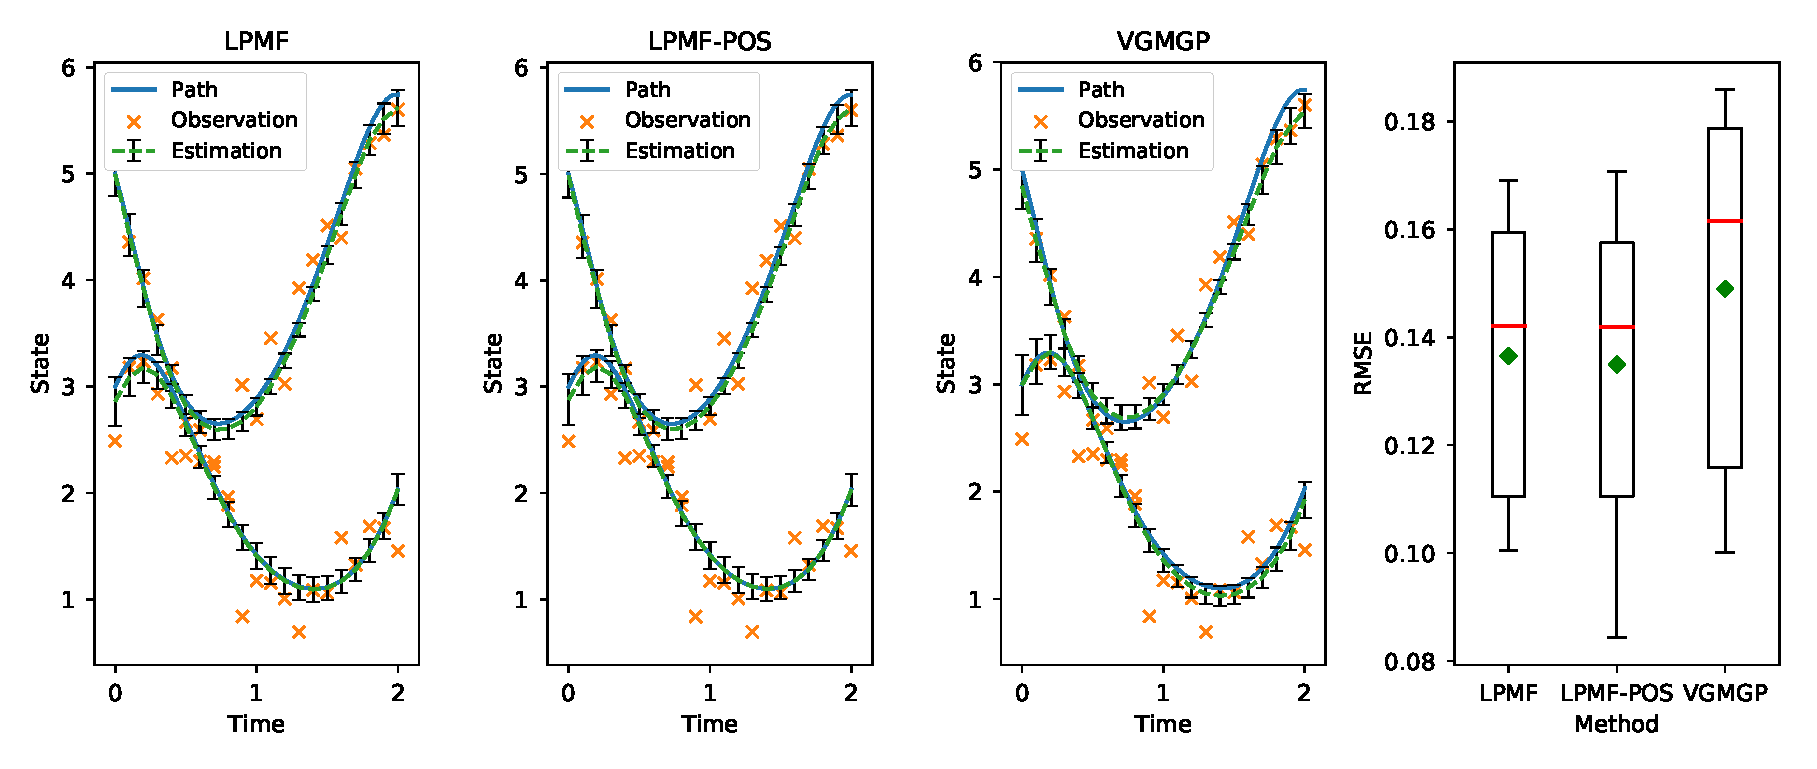
\includegraphics[width=\textwidth]{graphics/lotka-states}
        \label{fig-lotka-state}
    \end{figure}
\end{frame}

\begin{frame}[t]
    \frametitle{Parameter estimation}
    \begin{figure}
        \centering
        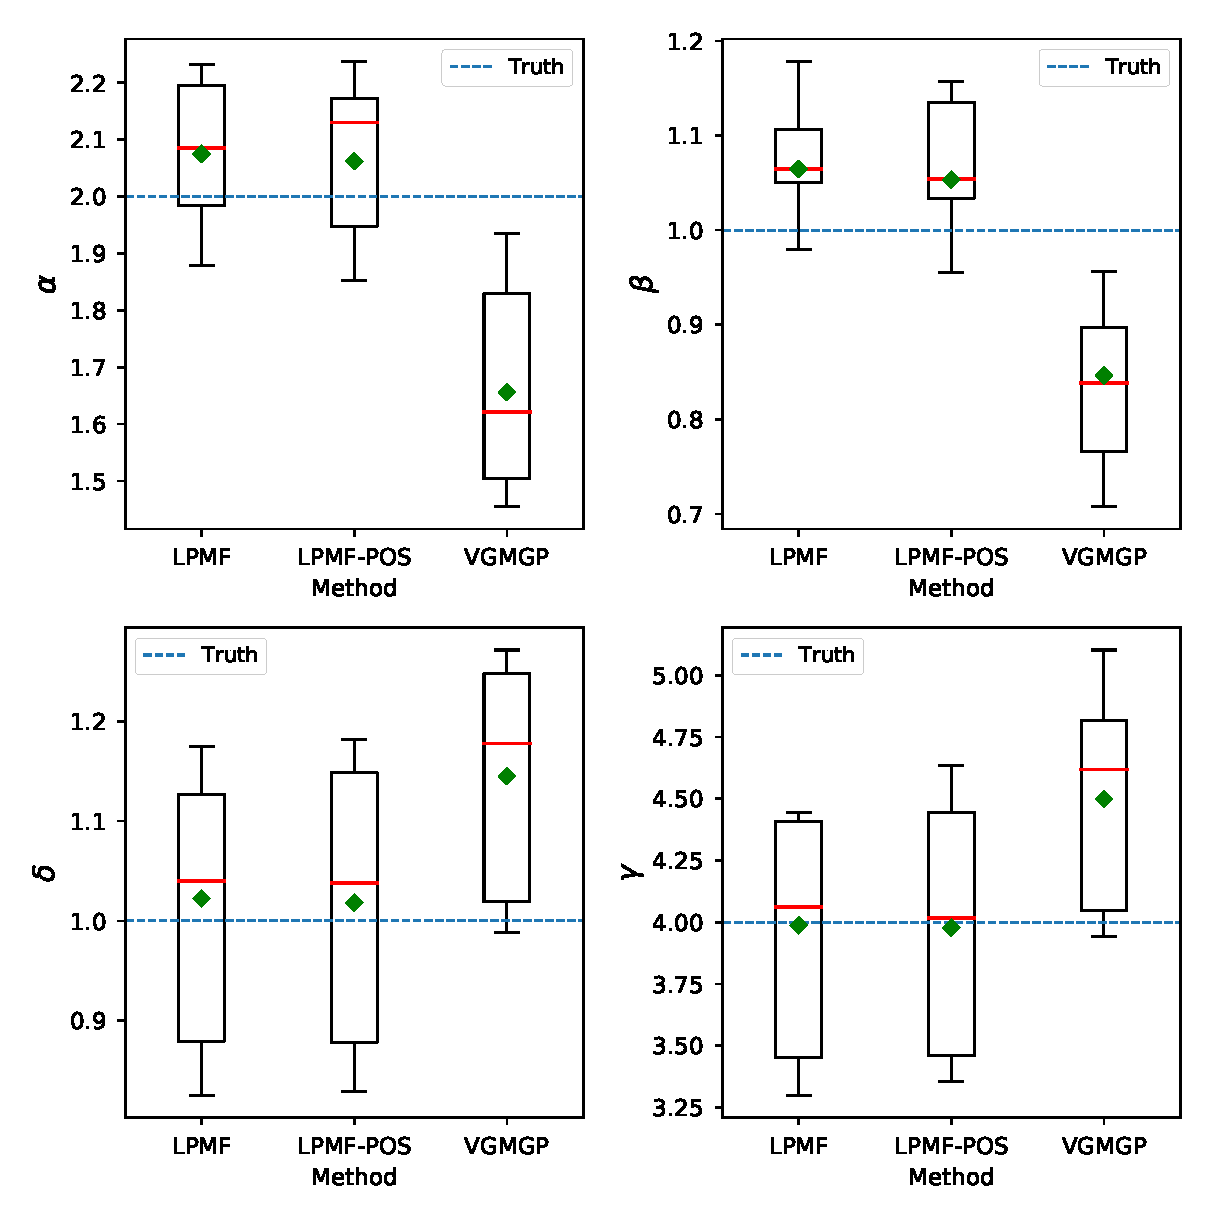
\includegraphics[width=1\textwidth]{graphics/lotka-parameters-boxplot}
        \label{fig-lotka-parameters-boxplot}
    \end{figure}
\end{frame}

\begin{frame}[t]
    \frametitle{Runtime performance}
    \begin{figure}
        \centering
        \includegraphics[width=0.45\textwidth]{graphics/lotka-runtime-boxplot}
        \label{fig-lotka-runtime-boxplot}
    \end{figure}                                       
\end{frame}

\begin{frame}[t]
    \frametitle{Positivity constraint on states}
    \begin{figure}
        \centering
        \includegraphics[width=\textwidth]{graphics/lotka-fail}
        \label{fig-lotka-fail}
    \end{figure}     
\end{frame}

\begin{frame}[t]
    \frametitle{Protein signalling transduction pathway}
    A signal transduction cascade model to describe the dynamics among protein species.
    \begin{align}
        \proteinSdt 
        & = 
        -\proteinki{1} \times \proteinS 
        -\proteinki{2} \times \proteinS \times \proteinR
        + \proteinki{3} \times \proteinRS
        \nonumber
        \\
        \proteindSdt
        & = 
        \proteinki{1} \times \proteinS    
        \nonumber
        \\
        \proteinRdt
        & =
        -\proteinki{2} \times \proteinS \times \proteinR 
        + \proteinki{3} \times \proteinRS
        + \proteinV \times \frac{\proteinRpp}{\proteinKm + \proteinRpp}
        \nonumber
        \\
        \proteinRSdt
        & =
        \proteinki{2} \times \proteinS \times \proteinR
        - \proteinki{3} \times \proteinRS
        - \proteinki{4} \times \proteinRS
        \nonumber
        \\
        \proteinRppdt 
        & =
        \proteinki{4} \times \proteinRS - \proteinV \times \frac{\proteinRpp}{\proteinKm + \proteinRpp}
    \end{align}
    where 
    \begin{itemize}
        \item[] $\proteinS, \proteindS, \proteinR, \proteinRS, \proteinRpp \ \in \R_{\geqslant 0}$ are the concentrations of proteins. 
        \item[] $\proteinki{1}, \proteinki{2}, \proteinki{3}, \proteinki{4}, \proteinKm, \proteinV \in \R^+$ are kentic parameters
    \end{itemize}
\end{frame}

\begin{frame}[t]
    \frametitle{Experimental setup}
    \begin{table}
    \centering
    \label{table-protein-setup}
    \begin{tabular}{|c|c|c|c|c|c|c|c|c|}
    \hline
    $K$ & $K_{obs}$ & $t_0$ & $t_T$ & $\delta t$ & $k_1, k_2, k_3, k_4, V, Km$ & $\dymsigmak{k}^2$ \\ \hline
    5 & 4 & 0 & 100 & 0.05 & 0.07, 0.6, 0.05, 0.3, 0.017, 3 & 0.01\\ \hline
    \end{tabular}
    \end{table}    
    
    \vspace{\baselineskip}
    The observations, in total 15, are collected at time points 0, 1, 2, 4, 5, 7, 10, 15, 20, 30, 40, 50, 60, 80 and 100.
\end{frame}

\begin{frame}[t]
    \frametitle{State estimation}
    \begin{figure}
        \centering
        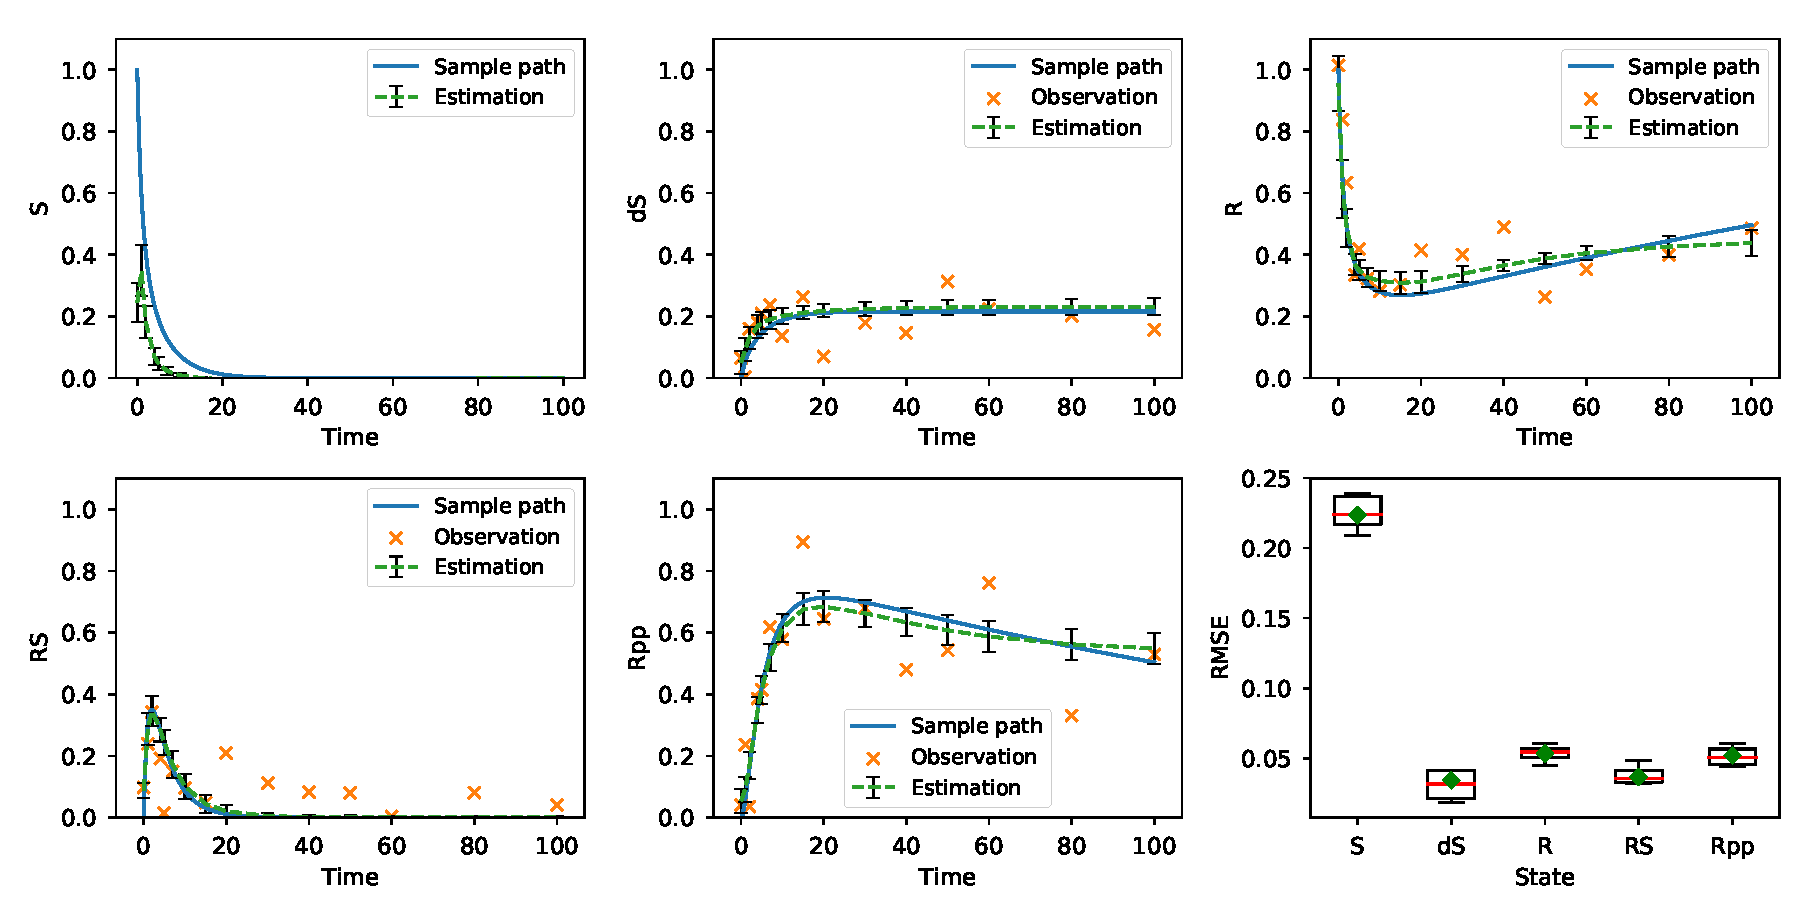
\includegraphics[width=0.9\textwidth]{graphics/protein-states-without-km-partial}
        \label{fig-protein-states-partial-without-km}
    \end{figure}
\end{frame}

\begin{frame}[t]
    \frametitle{Parameter estimation}
    \begin{figure}
        \centering
        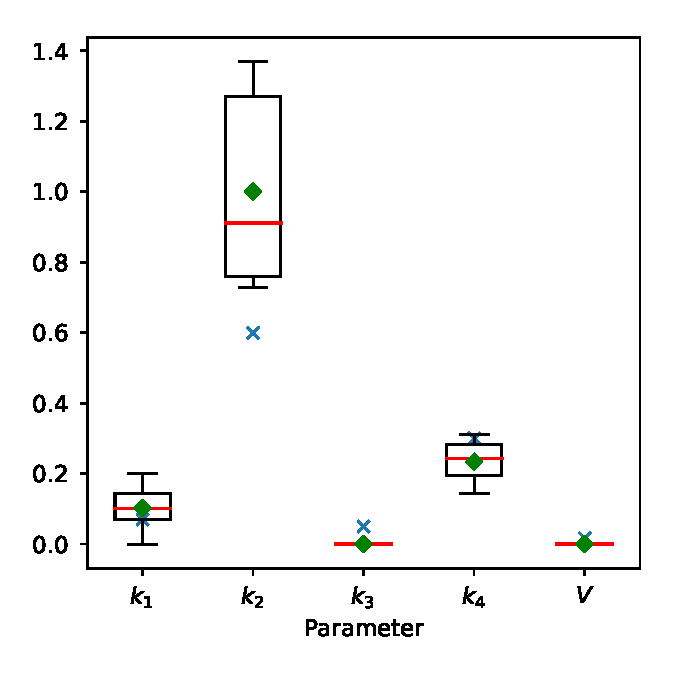
\includegraphics[width=0.4\textwidth]{graphics/protein-parameters-without-km-partial}
        \label{fig-protein-parameters-partial-without-km}
    \end{figure}            
\end{frame}

\begin{frame}[t]
    \frametitle{Lorenz 96 model}
    A minimalistic weather forecast model.
    A $K$-dimensional deterministic Lorenz 96 dynamical system is defined for $k = \mrange{1}{K}$, state-wise as follows:
    \begin{align}
        \dymdxktn{k}{}
         & = (\dymxktn{k+1}{} - \dymxktn{k-2}{})\dymxktn{k-1}{} - \dymxktn{k}{} + F
        \label{eq-lorenz-96-drift}
    \end{align}
    where
    \begin{align}
        \dymxktn{-1}{} & = \dymxktn{K-1}{}
        \nonumber
        \\
        \dymxktn{0}{} & = \dymxktn{K}{}
        \nonumber
        \\
        \dymxktn{K+1}{} & =\dymxktn{1}{}        
        \nonumber
    \end{align}
    \begin{align}
        F \in \R \text{ controls the behavior of the system}
    \end{align}
\end{frame}

\begin{frame}[t]
    \frametitle{Experimental setup}
    \begin{table}
        \centering
        \label{table-lorenz-96-setup}
        \begin{tabular}{|c|c|c|c|c|c|c|c|c|}
        \hline
        $K$ & $K_{obs}$ & $t_0$ & $t_T$ & $\delta t$ & $F$ & $\dymsigmak{k}^2$  & $\sderhoq{k}^2$ & $freq_{obs}$ \\ \hline
        500 & 325 (65\%) & 0 & 4 & 0.01 & 8 & 1 & 4 & 8 \\ \hline
        \end{tabular}
    \end{table}
\end{frame}

\begin{frame}[t]
    \frametitle{State estimation}
    \begin{figure}
        \centering
        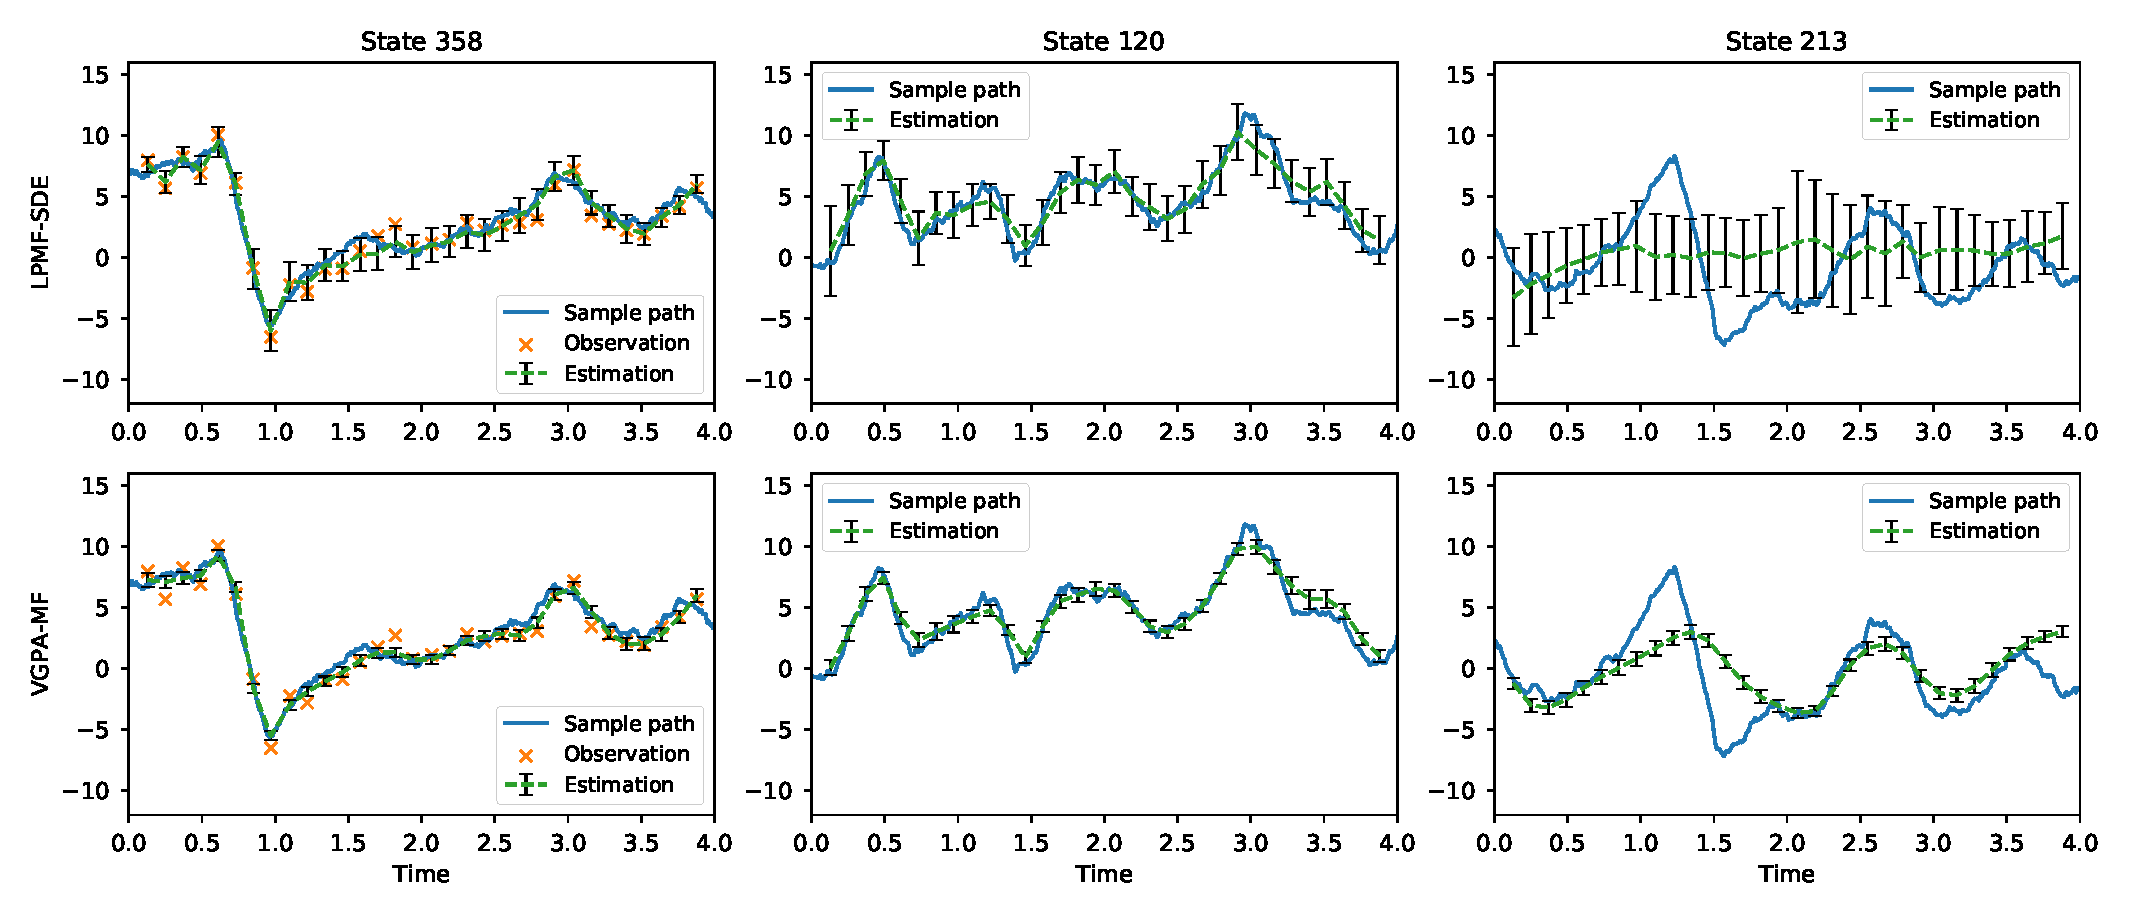
\includegraphics[width=\textwidth]{graphics/lorenz-96-states}
        \label{fig-lorenz-96-states}
    \end{figure}
\end{frame}

\begin{frame}[t]
    \frametitle{State estimation}
    \begin{figure}
        \centering
        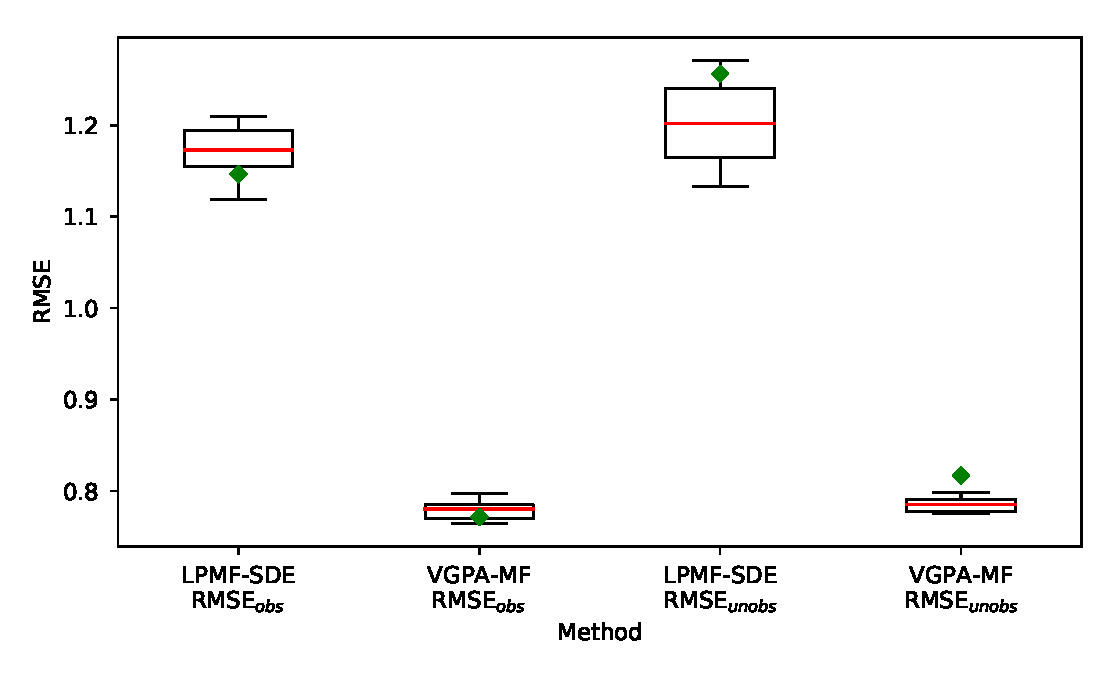
\includegraphics[width=0.7\textwidth]{graphics/lorenz-96-states-boxplot}    
        \label{fig-lorenz-96-state-boxplot}
    \end{figure}
\end{frame}

\begin{frame}[t]
    \frametitle{Parameter estimation}
    \begin{figure}
        \centering
        \begin{subfigure}[b]{0.32\textwidth}
            \includegraphics[width=\linewidth]{graphics/lorenz-96-parameters}
            \label{fig-lorenz-96-parameters}
        \end{subfigure}
        \begin{subfigure}[b]{0.32\textwidth}
            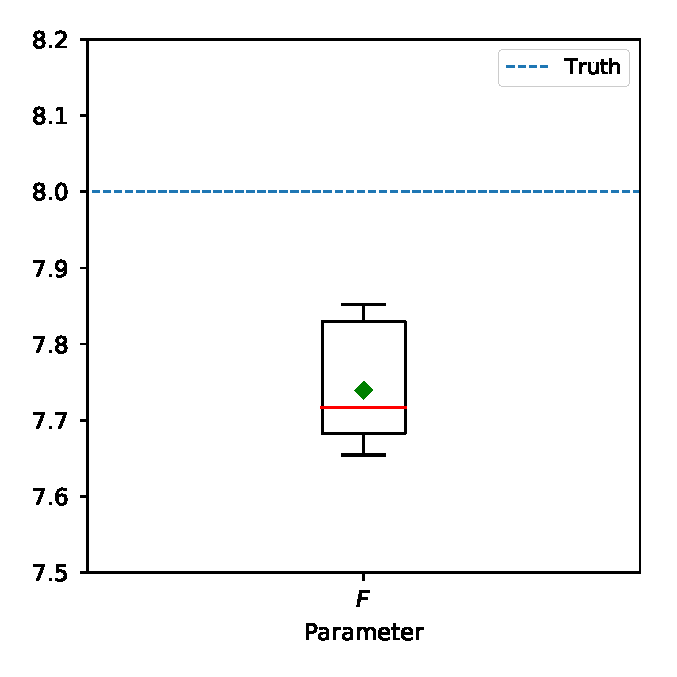
\includegraphics[width=\linewidth]{graphics/lorenz-96-parameters-boxplot}
            \label{fig-lorenz-96-parameters-boxplot}
        \end{subfigure}
        \begin{subfigure}[b]{0.32\textwidth}
            \includegraphics[width=\textwidth]{graphics/lorenz-96-parameters-grid-search}
            \label{fig-lorenz-96-parameters-grid-search}
        \end{subfigure}
        \label{fig-lorenz-96-parameters-group}    
    \end{figure}
\end{frame}

\begin{frame}[t]
    \frametitle{Runtime performance}
    \begin{figure}
        \centering
        \begin{subfigure}[b]{0.42\textwidth}
            \includegraphics[width=\textwidth]{graphics/lorenz-96-runtime-boxplot}
            \label{fig-lorenz-96-runtime-boxplot}
        \end{subfigure}
        \begin{subfigure}[b]{0.56\textwidth}
        \includegraphics[width=\textwidth]{graphics/lorenz-96-scalability}
        \label{fig-lorenz-96-scalability}
        \end{subfigure}  
    \end{figure}    
\end{frame}

\begin{frame}[t]
    \frametitle{Lorenz 63 model}
    Low dimensional mathematical model for thermal convection in the atmosphere.
    The vector field of the deterministic Lorenz 63 is defined as follows:
    \begin{align}
        \dymf
        & =
        \begin{bmatrix}
            \dot{x}(t)
            \\ 
            \dot{y}(t)
            \\
            \dot{z}(t)
        \end{bmatrix}
        =
        \begin{bmatrix}
            \sigma(y(t) - x(t))
            \\
            x(t)(\rho - z(t)) - y(t)
            \\
            x(t)y(t) - \beta z(t)
        \end{bmatrix}
        \label{eq-lorenz-63-odes}
    \end{align}
    where
    \begin{itemize}
        \item[] $\dymx = [x(t), y(t), z(t)]^\top \in \R^3$ is the state vector.
        \item[] $\dymtheta = [\sigma, \rho, \beta]^\top \in \R^3$ is the parameter vector
    \end{itemize}
\end{frame}

\begin{frame}[t]
    \frametitle{Experimental setup}
    \begin{table}
    \centering
    \label{table-lorenz-63-setup}
    \begin{tabular}{|c|c|c|c|c|c|c|c|c|}
    \hline
    $K$ & $K_{obs}$ & $t_0$ & $t_T$ & $\delta t$ & $\sigma, \rho, \beta$ & $\dymsigmak{k}^2$  & $\sderhoq{k}^2$ & $freq_{obs}$ \\ \hline
    3 & 3 or 2 & 0 & 20 & 0.01 & $10, 28, \frac{8}{3}$ & 2 & 10 & 5 \\ \hline
    \end{tabular}
    \end{table}    
\end{frame}

\begin{frame}[t]
    \frametitle{Sample path}
    \begin{figure}
        \centering
        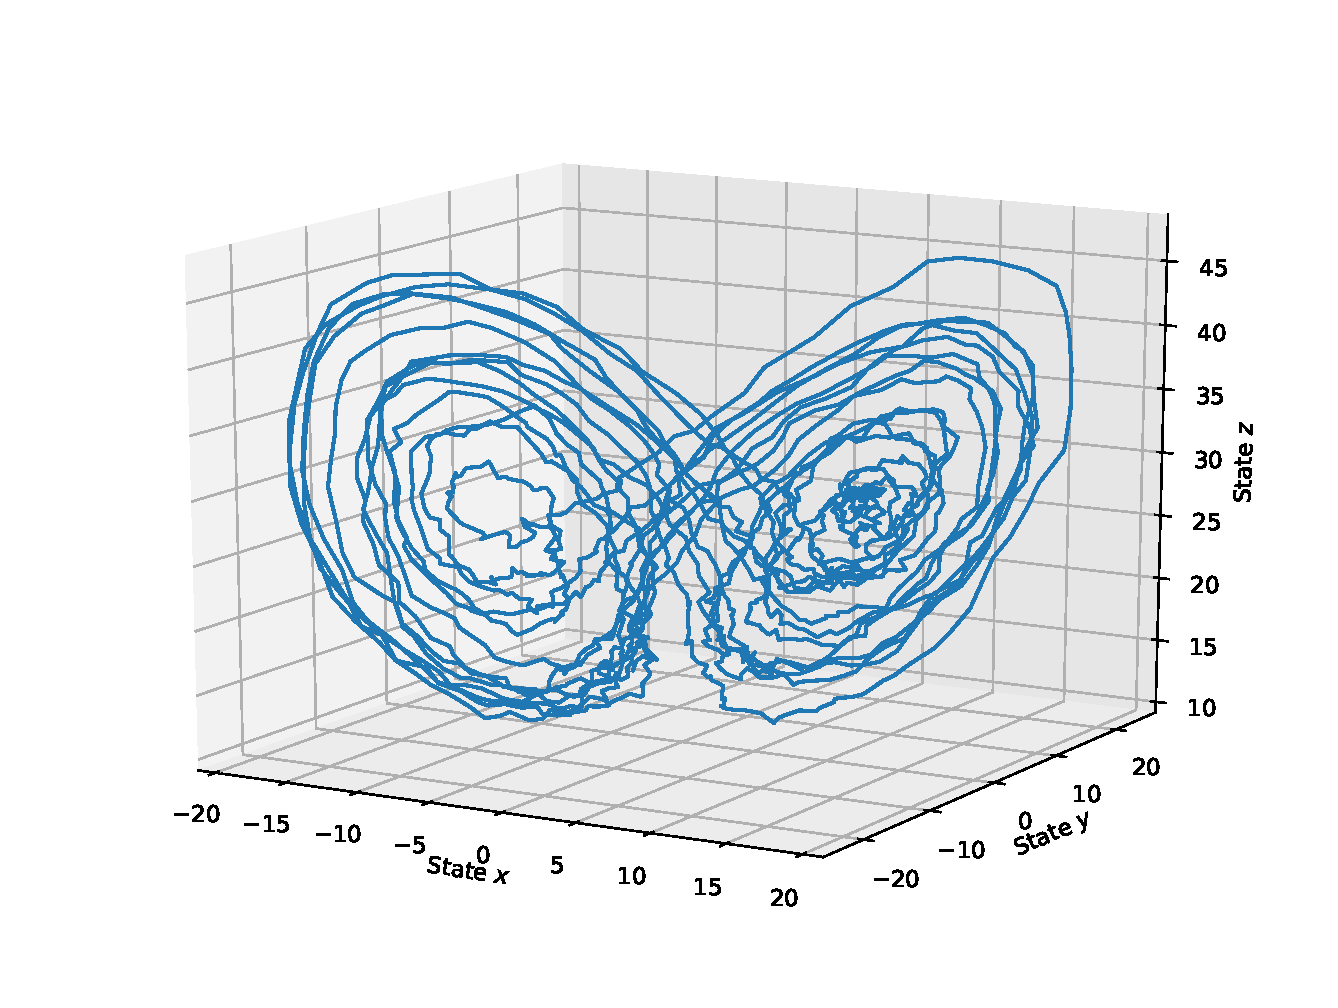
\includegraphics[width=0.6\textwidth]{graphics/lorenz-63-sample-path}
        \label{fig-lorenz-63-sample-path}
    \end{figure}    
\end{frame}

\begin{frame}[t]
    \frametitle{State estimation}
    \begin{figure}
        \centering
        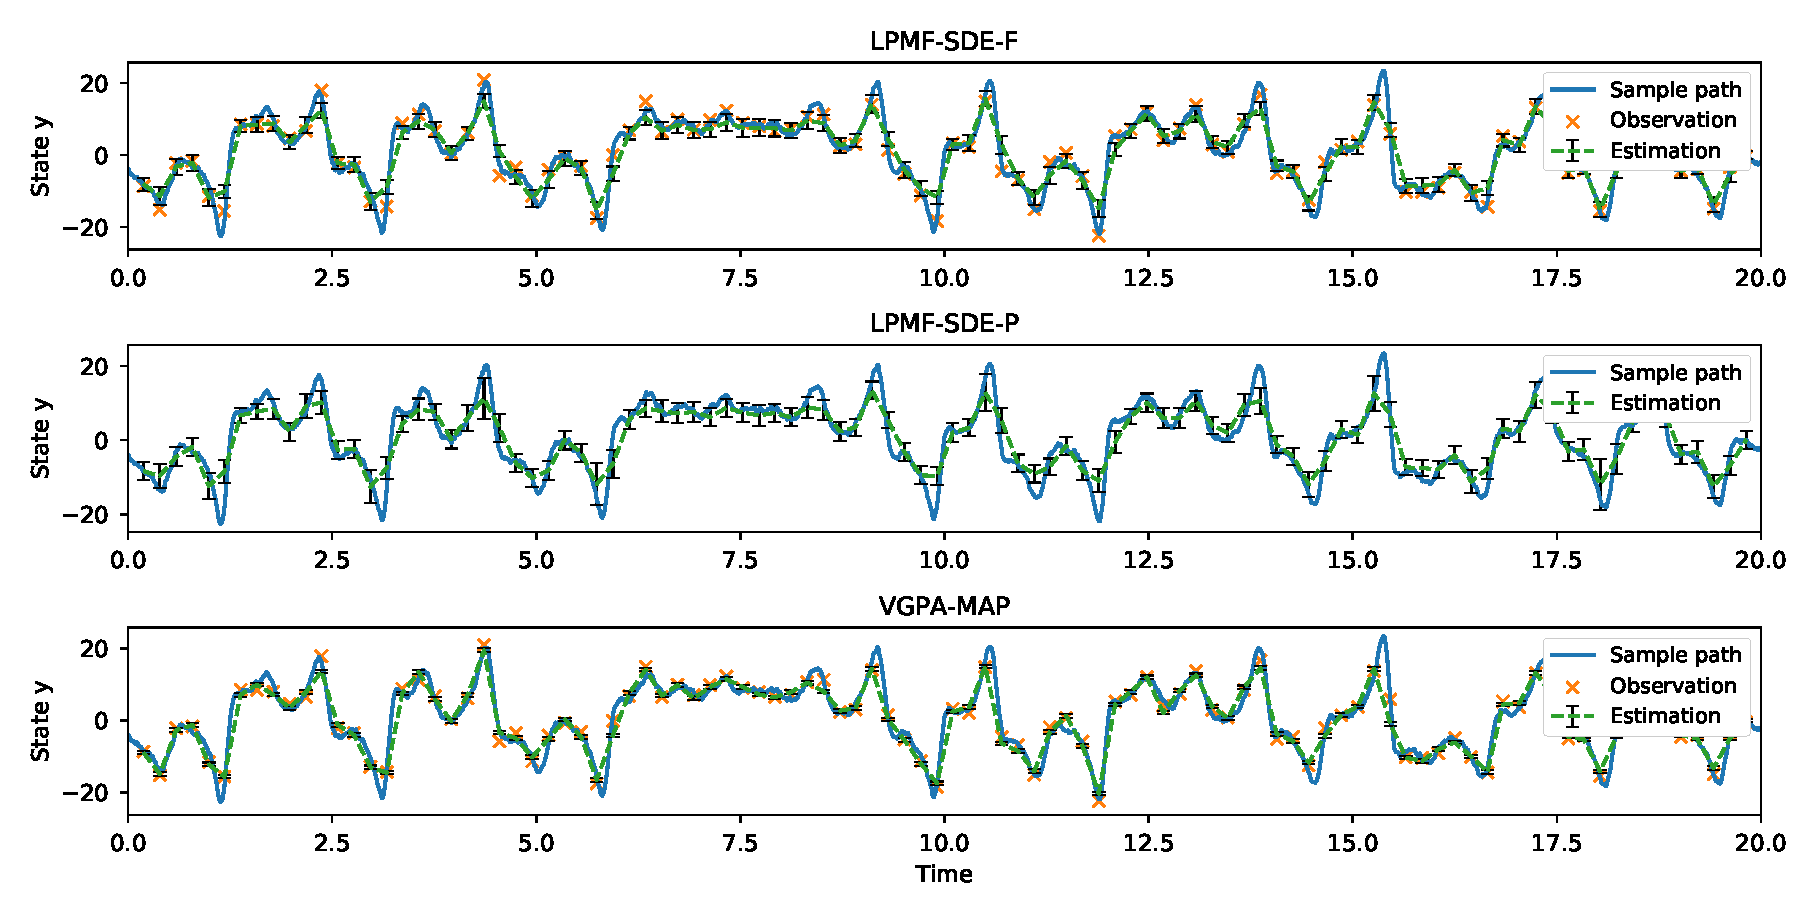
\includegraphics[width=0.95\textwidth]{graphics/lorenz-63-states}
        \label{fig-lorenz-63-states}
    \end{figure}
\end{frame}

\begin{frame}[t]
    \frametitle{State estimation}
    \begin{figure}
        \centering
        \includegraphics[width=0.7\linewidth]{graphics/lorenz-63-states-boxplot}
        \label{fig-lorenz-63-state-boxplot}
    \end{figure}            
\end{frame}

\begin{frame}[t]
    \frametitle{Parameter estimation}
    \begin{figure}
        \centering
        \begin{subfigure}{0.24\textwidth}
            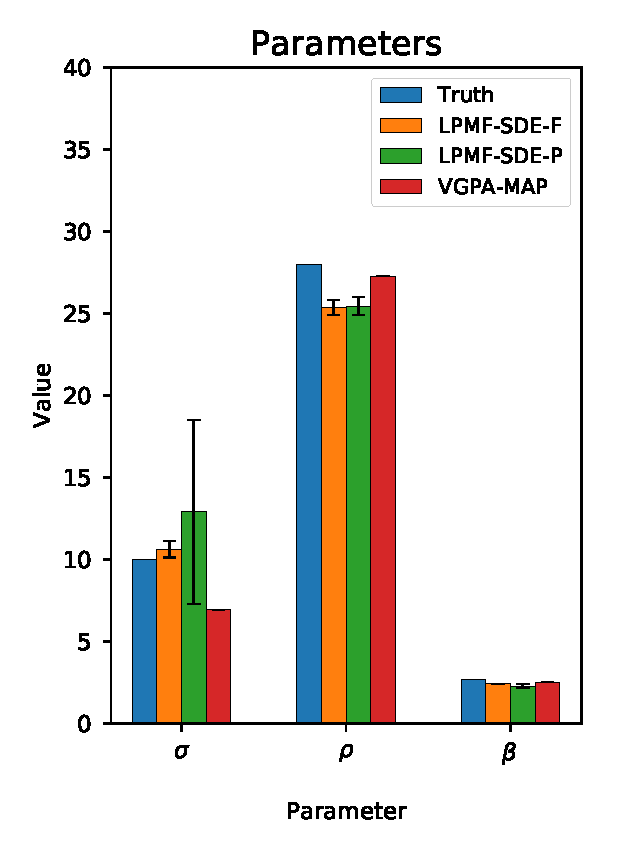
\includegraphics[width=\linewidth]{graphics/lorenz-63-parameters}
            \label{fig-lorenz-63-parameters}
        \end{subfigure}
        \begin{subfigure}{0.24\textwidth}
            \includegraphics[width=\linewidth]{graphics/lorenz-63-parameters-sigma-boxplot}
            \label{fig-lorenz-63-parameters-sigma-boxplot}
        \end{subfigure}
        \begin{subfigure}{0.24\textwidth}
            \includegraphics[width=\linewidth]{graphics/lorenz-63-parameters-rho-boxplot}
            \label{fig-lorenz-63-parameters-rho-boxplot}
        \end{subfigure}
        \begin{subfigure}{0.24\textwidth}
            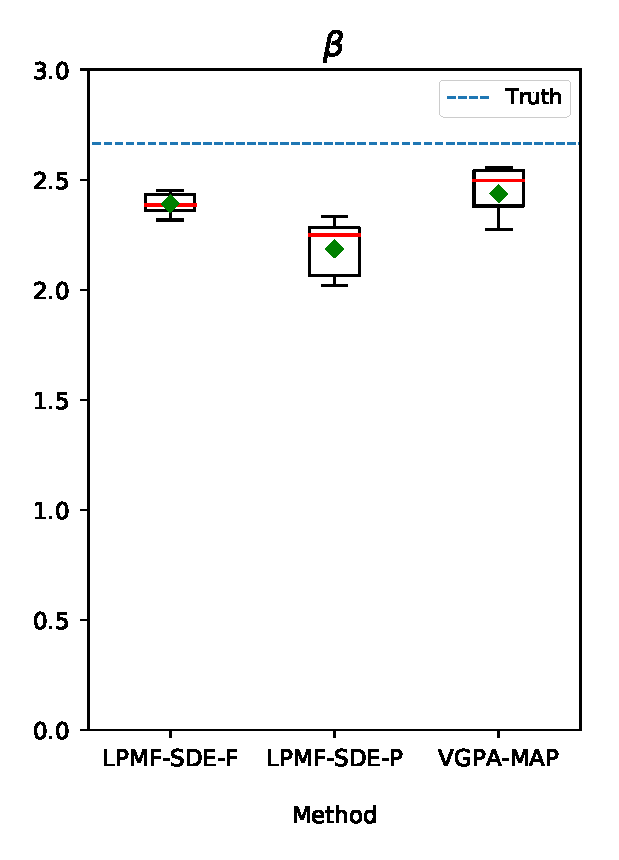
\includegraphics[width=\linewidth]{graphics/lorenz-63-parameters-beta-boxplot}
            \label{fig-lorenz-63-parameters-beta-boxplot}
        \end{subfigure}
        \label{fig-lorenz-63-parameters-group}
    \end{figure}    
\end{frame}

\begin{frame}[t]
    \frametitle{Parameter estimation}
	\begin{figure}
	    \centering
	    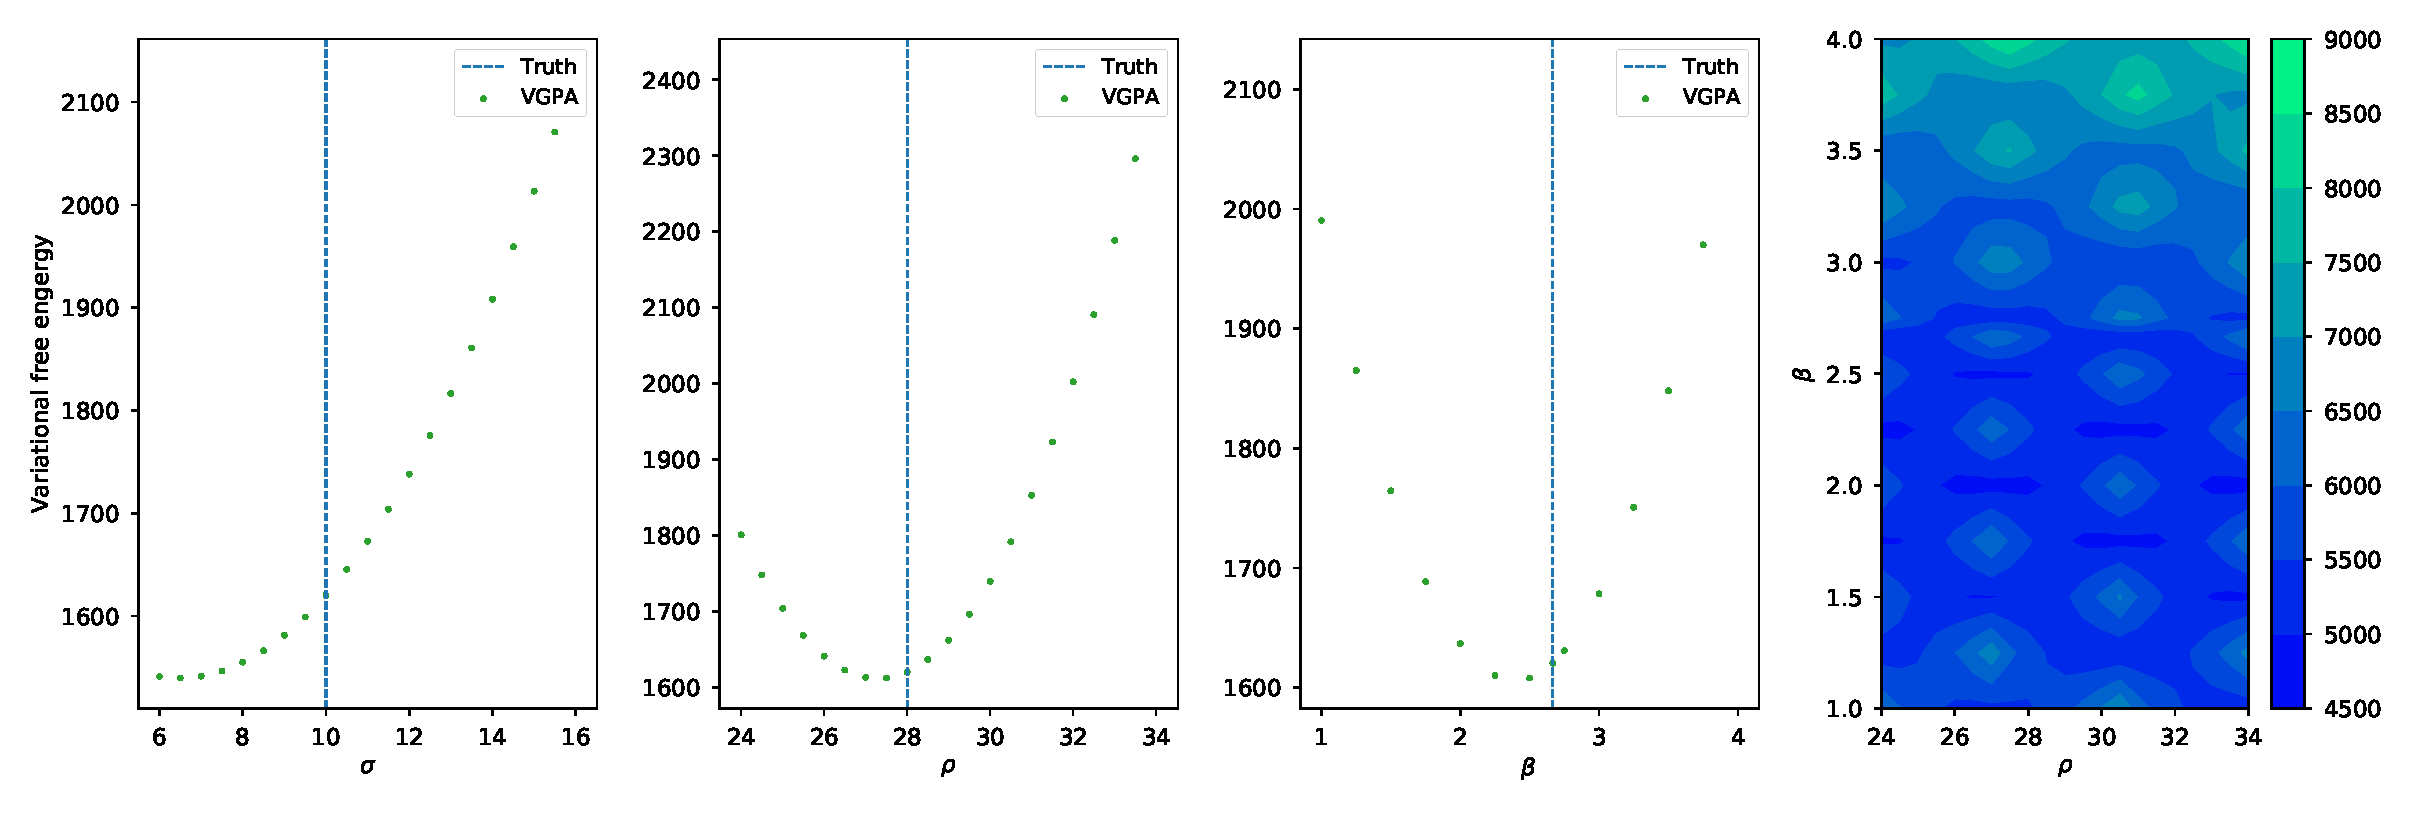
\includegraphics[width=\linewidth]{graphics/lorenz-63-parameters-grid-search}
	    \label{fig-lorenz-63-parameters-grid-search}    
	\end{figure} 
\end{frame}

\begin{frame}[t]
    \frametitle{Runtime performance}
    \begin{figure}
        \centering
        \includegraphics[width=0.7\linewidth]{graphics/lorenz-63-runtime-boxplot}
        \label{fig-lorenz-63-runtime-boxplot}    
    \end{figure}
\end{frame}
\chapter{Conclusion}
\label{ch-conclusion}

This work examines the problem of state and parameter estimation in deterministic and random dynamical systems given noisy, sparse or even incomplete observations.
A mean-field Laplace approximation solution is proposed to address the intractability of the posterior distribution and has been shown empirically to be robust and scalable.
Further, it relaxes the structural assumption imposed on the dynamical systems from previous work and introduces positivity constraints on the states and parameters.
Based on the correspondence between RODEs and SDEs, a highly efficient parallel inference technique is devised to address problems involving diffusion processes.

%\begin{frame}[t]
    \frametitle{Preliminary: Gaussian process regression}
    A \emph{Gaussian process (GP)} is a collection of random variables such that any finite subset of it forms a multivariate Gaussian distribution.
    
    \vspace{\baselineskip}
    \textbf{GP regression}
    \begin{itemize}
        \item A nonparametric, kernel-based Bayesian regression technique.
        \item In application, 
        \begin{itemize}
            \item Specify a GP prior on the regression function.
            \item Convert the prior into posterior after observing data to make prediction.
        \end{itemize}
    \end{itemize}
\end{frame}

\begin{frame}[t]
    \frametitle{Preliminary: Gaussian process regression}    
    The GP prior on $f$ is denoted as
    \begin{align}
        f(\mvector{x}{}) & \sim \mathcal{GP}(m(\mvector{x}),\ k(\mvector{x},\ \mvector{x}^\prime)) 
        \label{eq-gp}
        \\
        \intertext{where}
        m(\mvector{x}) &= \mathbb{E}[f(\mvector{x})]
        \nonumber
        \\  		
        k(\mvector{x}, \mvector{x}^\prime) &= \mathbb{E}[(f(\mvector{x}) - m(\mvector{x}))(f(\mvector{x}^\prime) - m(\mvector{x}^\prime))]
        \nonumber
    \end{align}    
    
    \vspace{\baselineskip}
    For any finite collection $\mdata{X} = \{\mvector{x}_i \in \R^D \vert i=\mrange{1}{N}\}$, we have
    \begin{align}
        \mdata{f} \vert \mdata{X} \sim \mathcal{N}(\mdata{m},\ \mdata{K}(\mdata{X},\ \mdata{X}))        
    \end{align}
    where $\mathrm{f}_i = f(\mvector{x}_i)$, $\mathrm{m}_i = m(\mvector{x}_i)$, and $\mathrm{K}_{ij} = k(\mvector{x}_i, \mvector{x}_j)$ for $i, j=\mrange{1}{N}$.
\end{frame}

\begin{frame}[t]
    \frametitle{Preliminary: Gaussian process regression}
    Assuming i.i.d.\ additive white Gaussian noise $\epsilon \sim \mathcal{N}(0, \sigma^2)$ such that $y_i = f(\mvector{x}_i) + \epsilon_i$ for $i=\mrange{1}{N}$, for any finite collection $\mdata{X}^* = \{\mvector{x}^*_i \in \R^D \vert i=\mrange{1}{M}\}$:
    \begin{align}
        \begin{bmatrix}
            \mdata{y} 
            \\ 
            \mdata{f}^*
        \end{bmatrix}
        \sim 
        \mathcal{N}(
            \begin{bmatrix}
                \mdata{m} 
                \\ 
                \mdata{m}^*
            \end{bmatrix}
            ,
            \begin{bmatrix}
                \mdata{K}(\mdata{X}, \mdata{X}) + \sigma^2\mI 
                    & \mdata{K}(\mdata{X}, \mdata{X}^*) 
                \\ 
                \mdata{K}(\mdata{X}^*, \mdata{X}) 
                    & \mdata{K}(\mdata{X}^*, \mdata{X}^*)
            \end{bmatrix}
        )
    \end{align}
    
    \vspace{\baselineskip}
    The noise-free posterior on $\mdata{f}^*$ is then 
    \begin{align}
        \mdata{f}^* \vert \mdata{X},\mdata{y},\sigma,\mdata{X}^*
        \sim
        \mathcal{N}(
            & \mdata{m}^* 
            + \mdata{K}(\mdata{X}^*, \mdata{X})[\mdata{K}(\mdata{X}, \mdata{X}) + \sigma^2\mI]^{-1}(\mdata{y} - \mdata{m}),
            \nonumber
            \label{eq-gp-posterior}
            \\        
            & \mdata{K}(\mdata{X}^*, \mdata{X}^*) 
            - \mdata{K}(\mdata{X}^*, \mdata{X})[\mdata{K}(\mdata{X}, \mdata{X}) + \sigma^2\mI]^{-1}\mdata{K}(\mdata{X}, \mdata{X}^*)
        )
    \end{align}
\end{frame}

\end{document}
